% =============================================================
% บทที่ 4 - การวิเคราะห์ระบบ และการพัฒนาโปรแกรม
% เนื้อหาหลักเรียบเรียงจาก Research Me (1).docx (บทที่ 4 การวิเคราะห์ระบบ และการพัฒนาโปรแกรม)
% หมายเหตุ: แผนภาพ (Use Case / SSD / Sequence / Activity / ER / Mockup) จับคู่ไฟล์ภาพจริง
% จาก Research Me (1).docx แล้ว (report/images/diagram-*.png) ยกเว้น System Sequence Diagram
% แบบรวม 3 ฟังก์ชัน (แชตบอต/ค้นหาข้อมูล/สร้างแผนการเดินทาง) ที่ยังไม่มีภาพต้นฉบับ -- คงกรอบ
% placeholder ไว้ก่อน
% =============================================================

การพัฒนาแอปพลิเคชันส่วนกลางสำหรับการท่องเที่ยวในจังหวัดขอนแก่น (Dino) มุ่งเน้นการใช้เทคโนโลยีปัญญาประดิษฐ์เชิงสร้างสรรค์ (Generative AI) เพื่อแก้ปัญหาความซับซ้อนในการวางแผนการเดินทาง โดยเปลี่ยนจากการใช้อัลกอริทึมแบบดั้งเดิมมาเป็นการใช้ LLM ร่วมกับฐานข้อมูลเวกเตอร์ในการประมวลผล ผลการวิเคราะห์และพัฒนาระบบมีรายละเอียดดังต่อไปนี้

% -----------------------------------------------------------
\section{การวิเคราะห์ระบบ}
% -----------------------------------------------------------

\subsection{การวิเคราะห์ปัญหาและการทำงานเดิม}

\subsubsection{ปัญหาการวางแผนการท่องเที่ยว}

ปัญหาสำคัญในปัจจุบันคือการเข้าถึงข้อมูลการท่องเที่ยวที่กระจัดกระจายอยู่ในหลายช่องทาง เช่น เว็บไซต์ หน่วยงานราชการ เพจโซเชียลมีเดีย หรือแอปพลิเคชันทั่วไป นักท่องเที่ยวจำเป็นต้องใช้เวลาค้นหาข้อมูลจากหลายแหล่ง ซึ่งมักพบปัญหาว่าข้อมูลไม่ครบถ้วน ไม่ทันสมัย นอกจากนี้ แหล่งข้อมูลที่มีอยู่ในปัจจุบันมิได้ถูกรวบรวมอย่างเป็นระบบ ทำให้นักท่องเที่ยวประสบความยากลำบากในการเข้าถึงข้อมูลเพื่อใช้ในการวางแผนการเดินทางให้สอดคล้องกับความสนใจและงบประมาณของตนเอง

\subsubsection{การทำงานเดิม}

กระบวนการทำงานแบบดั้งเดิม (Manual Process) กำหนดให้นักท่องเที่ยวต้องดำเนินการสืบค้นและประมวลผลข้อมูลด้วยตนเองผ่านขั้นตอนที่มีความซับซ้อนและใช้เวลามาก ดังนี้

\begin{enumerate}[label=(\arabic*)]
\item การสืบค้นข้อมูล นักท่องเที่ยวทำการค้นหาข้อมูลสถานที่ท่องเที่ยว ที่พัก และร้านอาหาร ผ่านแพลตฟอร์มต่าง ๆ ที่แยกส่วนกันและไม่มีการเชื่อมโยงข้อมูลอย่างเป็นระบบ
\item การตรวจสอบเส้นทางและระยะเวลา นักท่องเที่ยวต้องนำรายการสถานที่ที่สนใจไปสืบค้นต่อในระบบภูมิสารสนเทศหรือแอปพลิเคชันแผนที่ เพื่อคำนวณระยะทางและประเมินระยะเวลาในการเดินทาง
\item การจัดตารางเวลาและงบประมาณ นักท่องเที่ยวต้องทำการคำนวณค่าใช้จ่ายและจัดลำดับแผนการเดินทางด้วยตนเอง (Manual Scheduling) ซึ่งมีโอกาสเกิดข้อผิดพลาดและสร้างความยุ่งยากในเชิงปฏิบัติ
\end{enumerate}

\subsection{ความต้องการของระบบ}

การวิเคราะห์ความต้องการของระบบถูกแบ่งออกเป็น 2 ส่วนหลัก ได้แก่ ความต้องการเชิงหน้าที่ที่ระบบต้องตอบสนองต่อผู้ใช้งาน และความต้องการที่ไม่ใช่เชิงหน้าที่ซึ่งเป็นตัวกำหนดมาตรฐานและคุณภาพของระบบ

\subsubsection{ความต้องการเชิงฟังก์ชัน}

ความต้องการในส่วนนี้ระบุถึงฟังก์ชันการทำงานหลักที่ระบบแอปพลิเคชันศูนย์กลางการท่องเที่ยวต้องสามารถดำเนินการได้ เพื่อรองรับการใช้งานของนักท่องเที่ยวและผู้ดูแลระบบ แสดงดังตารางที่ \ref{tab:func_req}

\begin{table}[H]
\centering
\caption{ความต้องการเชิงฟังก์ชัน (Functional Requirements)}
\label{tab:func_req}
\begin{tabular}{|c|p{4cm}|p{7cm}|}
\hline
\textbf{รหัส} & \textbf{ชื่อความต้องการ} & \textbf{รายละเอียดความต้องการ} \\
\hline
FR-01 & ระบบจัดการและแสดงผลข้อมูลการท่องเที่ยว & ระบบต้องสามารถแสดงรายละเอียดของสถานที่ท่องเที่ยวและกิจกรรม และอนุญาตให้นักท่องเที่ยวค้นหาข้อมูลตามหมวดหมู่ได้ \\ \hline
FR-02 & ระบบสร้างแผนการเดินทางอัตโนมัติ & ระบบต้องรับข้อมูลเงื่อนไขจากผู้ใช้ ได้แก่ วัน เวลา สถานที่ ความสนใจ งบประมาณ ความเร็วของทริป และประมวลผลเพื่อสร้างแผนการเดินทาง (Trip Planning) ที่จัดเรียงลำดับสถานที่และเวลาได้อย่างเหมาะสมแบบอัตโนมัติ \\ \hline
FR-03 & ระบบผู้ช่วยเสมือนอัจฉริยะ (แชตบอต) & ระบบต้องมีแชตบอตที่ขับเคลื่อนด้วย LLM เพื่อรับคำสั่ง วิเคราะห์บริบท และโต้ตอบให้คำแนะนำด้านการท่องเที่ยวกับผู้ใช้งานผ่านทางเว็บไซต์ \\ \hline
FR-04 & ระบบจัดการส่วนหลังบ้าน (Back-office) & ระบบต้องมีส่วนให้ผู้ดูแลระบบเข้าสู่ระบบเพื่อดำเนินการจัดการฐานข้อมูล (CRUD) สำหรับเพิ่ม ลบ แก้ไข และอัปเดตข้อมูลสถานที่ท่องเที่ยวและกิจกรรมได้ \\ \hline
FR-05 & ระบบสะสมและแลกพอยท์ (QR \& Rewards) & ระบบต้องอนุญาตให้ผู้ดูแลระบบผูก QR Code เข้ากับสถานที่พร้อมกำหนดจำนวนพอยท์ และจัดการรายการของรางวัลที่แลกได้ (CRUD) ส่วนฝั่งนักท่องเที่ยวต้องสามารถสแกน QR เพื่อสะสมพอยท์และนำพอยท์ไปแลกของรางวัลได้ \\ \hline
FR-06 & ระบบช่วยจัดการเนื้อหาด้วย AI (AI-Assisted Content) & ระบบต้องมีเครื่องมือช่วยผู้ดูแลระบบ ได้แก่ การดึงข้อมูลกิจกรรมจากข้อความโพสต์ (เช่น Facebook) มาเติมฟอร์มอัตโนมัติด้วย LLM และการสร้างคำอธิบายสถานที่ (Description) แบบเจาะจงรายสถานที่ด้วย AI \\
\hline
\end{tabular}
\end{table}

\subsubsection{ความต้องการที่ไม่ใช่เชิงฟังก์ชัน}

ความต้องการส่วนนี้ครอบคลุมถึงข้อจำกัดทางสถาปัตยกรรมและคุณสมบัติด้านประสิทธิภาพของระบบ เพื่อให้ระบบปัญญาประดิษฐ์และซอฟต์แวร์ทำงานได้อย่างมีเสถียรภาพ แสดงดังตารางที่ \ref{tab:nonfunc_req}

\begin{table}[H]
\centering
\caption{ความต้องการที่ไม่ใช่เชิงฟังก์ชัน (Non-Functional Requirements)}
\label{tab:nonfunc_req}
\begin{tabular}{|c|p{4cm}|p{7cm}|}
\hline
\textbf{รหัส} & \textbf{ชื่อความต้องการ} & \textbf{รายละเอียดความต้องการ} \\
\hline
NFR-01 & สถาปัตยกรรมและการรองรับการขยายตัว & ระบบต้องได้รับการออกแบบด้วยสถาปัตยกรรมไมโครเซอร์วิส เพื่อให้แต่ละส่วนทำงานแยกกันอย่างอิสระ และรองรับการขยายตัว (Scalability) เมื่อมีผู้ใช้งานเพิ่มขึ้น \\ \hline
NFR-02 & ความถูกต้องและความน่าเชื่อถือของ AI & ระบบ LLM ต้องมีกลไกลดการบิดเบือนข้อมูล (Hallucination) โดยทำงานร่วมกับระบบสืบค้นข้อมูล เพื่อบังคับให้อ้างอิงคำตอบจากฐานข้อมูลของระบบเป็นหลัก \\ \hline
NFR-03 & ประสิทธิภาพในการตอบสนอง (Performance) & ระบบต้องมีความหน่วงเวลา (Latency) ในการประมวลผลและส่งกลับคำตอบจากแชตบอตในระดับที่ต่ำ เพื่อให้การสนทนากับผู้ใช้เป็นไปอย่างราบรื่น \\ \hline
NFR-04 & ความปลอดภัยของข้อมูล (Security) & ระบบจัดการหลังบ้านต้องมีการยืนยันตัวตน (Authentication) และการกำหนดสิทธิ์ (Authorization) ที่รัดกุม เพื่อป้องกันการเข้าถึงหรือแก้ไขฐานข้อมูลโดยไม่ได้รับอนุญาต \\
\hline
\end{tabular}
\end{table}

\subsection{Use Case Diagram และรายละเอียด}

% คำสั่งวาด Actor แบบ UML (stick figure) ด้วย TikZ สำหรับ Use Case Diagram ทั้งสองภาพในหัวข้อนี้
\newcommand{\umlactor}[2]{%
  \begin{scope}[shift={(#1)}]
    \draw[thick] (0,1.05) circle (0.22);
    \draw[thick] (0,0.83) -- (0,0.25);
    \draw[thick] (-0.28,0.65) -- (0.28,0.65);
    \draw[thick] (0,0.25) -- (-0.28,-0.25);
    \draw[thick] (0,0.25) -- (0.28,-0.25);
    \node[font=\small, align=center, below=2pt] at (0,-0.25) {#2};
  \end{scope}
}

\begin{figure}[H]
\centering
\resizebox{0.98\linewidth}{!}{%
\begin{tikzpicture}[
  usecase/.style={ellipse, draw, thick, align=center, text width=3.3cm, minimum height=1.3cm, font=\small, inner sep=3pt},
  node distance=2.9cm and 2.7cm
]
\node[usecase] (uc01) {ถามตอบข้อมูลโดยใช้ แชตบอต\\(UC-01)};
\node[usecase, below=of uc01] (uc02) {ค้นหาข้อมูลสถานที่ท่องเที่ยว กิจกรรม และอีเวนท์\\(UC-02)};
\node[usecase, below=of uc02] (uc03) {สแกน QR Code เพื่อสะสมพอยท์\\(UC-03)};
\node[usecase, below=of uc03] (uc06) {สร้างแผนการเดินทาง\\(UC-06)};

\node[usecase, right=of uc02, yshift=1.0cm] (uc04) {ดูรายละเอียดข้อมูลสถานที่\\(UC-04)};
\node[usecase, right=of uc02, yshift=-1.0cm] (uc05) {ดูรายละเอียดข้อมูลอีเวนท์\\(UC-05)};

\node[usecase, right=of uc03] (uc08) {แลกของรางวัลด้วยพอยท์\\(UC-08)};

\node[usecase, right=of uc06, yshift=1.0cm] (uc064) {กรองสถานที่ตามขอบเขตพื้นที่\\(UC-06.4)};
\node[usecase, right=of uc06, yshift=-1.0cm] (uc07) {การปรับแผนการเดินทาง\\(UC-07)};

\draw[-{Stealth[length=2.5mm]}, dashed] (uc04) -- node[above,font=\scriptsize,fill=white,inner sep=1pt]{\guillemotleft extend\guillemotright} (uc02);
\draw[-{Stealth[length=2.5mm]}, dashed] (uc05) -- node[below,font=\scriptsize,fill=white,inner sep=1pt]{\guillemotleft extend\guillemotright} (uc02);
\draw[-{Stealth[length=2.5mm]}, dashed] (uc08) -- node[above,font=\scriptsize,fill=white,inner sep=1pt]{\guillemotleft extend\guillemotright} (uc03);
\draw[-{Stealth[length=2.5mm]}, dashed] (uc064) -- node[above,font=\scriptsize,fill=white,inner sep=1pt]{\guillemotleft extend\guillemotright} (uc06);
\draw[-{Stealth[length=2.5mm]}, dashed] (uc07) -- node[below,font=\scriptsize,fill=white,inner sep=1pt]{\guillemotleft extend\guillemotright} (uc06);

\node[draw, thick, inner sep=0.7cm, fit=(uc01)(uc02)(uc03)(uc06)(uc04)(uc05)(uc08)(uc064)(uc07)] (boundary) {};
\node[font=\bfseries\small, anchor=north] at (boundary.north) {\vphantom{Ay}Tourism Information System};

\umlactor{$(boundary.west)+(-1.9,0)$}{นักท่องเที่ยว\\(Tourist)}
\coordinate (tourist) at ($(boundary.west)+(-1.3,0.55)$);

\umlactor{$(boundary.east)+(1.9,-2.9)$}{ผู้ดูแลระบบ\\(Administrator)}
\coordinate (admin) at ($(boundary.east)+(1.5,-2.35)$);

\draw[thick] (tourist) -- (uc01);
\draw[thick] (tourist) -- (uc02);
\draw[thick] (tourist) -- (uc03);
\draw[thick] (tourist) -- (uc06);

\draw[thick] (admin) -- (uc08);
\end{tikzpicture}%
}
\caption{Tourist Use Case Diagram}
\label{fig:usecase_tourist}
\end{figure}

นักท่องเที่ยว (Tourist) เป็นผู้ใช้งานระดับทั่วไป (End-User) ของระบบสารสนเทศด้านการท่องเที่ยว ซึ่งมีบทบาทสำคัญในการเข้ามาปฏิสัมพันธ์กับระบบเพื่อสืบค้นข้อมูลและวางแผนการเดินทางตามความต้องการของตนเอง ผู้ใช้งานสามารถเรียกดูรายละเอียดข้อมูลกิจกรรมและสถานที่ท่องเที่ยวในเชิงลึก ค้นหาข้อมูลตามเงื่อนไขหรือความสนใจ สร้างแผนการเดินทาง (Trip Planning) ด้วยตนเอง และโต้ตอบกับระบบแชตบอตเพื่อสอบถามข้อมูลหรือขอคำแนะนำเพิ่มเติมได้แบบเรียลไทม์ รายละเอียดเชิงลึกของแต่ละฟังก์ชันแสดงในตารางที่ \ref{tab:uc01}--\ref{tab:uc08}

\begin{table}[H]
\centering
\caption{Use Case UC-01: ถามตอบข้อมูลโดยใช้ แชตบอต}
\label{tab:uc01}
\begin{tabular}{|p{3.2cm}|p{10cm}|}
\hline
\textbf{Use Case ID} & UC-01 \\ \hline
\textbf{Actor} & นักท่องเที่ยว (Tourist), KKU AI Gateway \\ \hline
\textbf{คำอธิบาย} & นักท่องเที่ยวสามารถโต้ตอบเพื่อสอบถามข้อมูลเกี่ยวกับการท่องเที่ยว สถานที่ กิจกรรมต่าง ๆ หรือฐานความรู้ที่ระบบมี ผ่านอินเทอร์เฟซแชตบอต โดยระบบจะส่งข้อความไปประมวลผลผ่าน KKU AI Gateway (เรียกใช้โมเดล Gemini แบบ OpenAI-compatible) เพื่อสร้างคำตอบที่ถูกต้องและเป็นธรรมชาติ \\ \hline
\textbf{เงื่อนไขเบื้องต้น} & ระบบเชื่อมต่อกับเครือข่ายอินเทอร์เน็ต และ KKU AI Gateway อยู่ในสถานะพร้อมใช้งาน \\ \hline
\textbf{กระแสหลัก (Main Flow)} & 1. นักท่องเที่ยวพิมพ์คำถามหรือข้อความลงในช่องแชทและกดส่ง \newline 2. ระบบรับข้อความและส่งต่อ (API Request) ไปยัง KKU AI Gateway โดยผ่าน RAG service เพื่อให้ได้ข้อมูลที่ตรงกับฐานข้อมูลที่มีอยู่ \newline 3. KKU AI Gateway ประมวลผลภาษาธรรมชาติและส่งคำตอบกลับมา (API Response) \newline 4. ระบบแสดงผลคำตอบบนหน้าจอแชตบอตให้นักท่องเที่ยวรับทราบ \\ \hline
\textbf{กระแสทางเลือก} & 3a. หากไม่สามารถเชื่อมต่อ KKU AI Gateway ได้ (เช่น Timeout) ระบบจะแสดงข้อความขออภัยและให้ผู้ใช้งานลองใหม่อีกครั้งในภายหลัง \\ \hline
\textbf{เงื่อนไขภายหลัง} & ข้อมูลการโต้ตอบถูกแสดงผลบนหน้าจอ แสดงประวัติการสนทนา และระบบพร้อมรับคำถามถัดไป \\
\hline
\end{tabular}
\end{table}

\begin{table}[H]
\centering
\caption{Use Case UC-02: ค้นหาข้อมูลสถานที่ท่องเที่ยว กิจกรรม และอีเวนท์}
\label{tab:uc02}
\begin{tabular}{|p{3.2cm}|p{10cm}|}
\hline
\textbf{Use Case ID} & UC-02 \\ \hline
\textbf{Actor} & นักท่องเที่ยว (Tourist) \\ \hline
\textbf{คำอธิบาย} & นักท่องเที่ยวสามารถสืบค้นข้อมูลด้านการท่องเที่ยวภายในระบบ โดยระบุคำค้นหาหรือตัวกรองที่ต้องการ เพื่อดูรายการสถานที่ กิจกรรม หรืออีเวนท์ที่สอดคล้องกับความสนใจ \\ \hline
\textbf{เงื่อนไขเบื้องต้น} & นักท่องเที่ยวอยู่ในหน้าแรก หรือหน้าสำหรับค้นหาข้อมูลของระบบ \\ \hline
\textbf{กระแสหลัก (Main Flow)} & 1. นักท่องเที่ยวระบุคำค้นหา หรือเลือกหมวดหมู่ที่ต้องการ (สถานที่, อีเวนท์) \newline 2. ระบบตรวจสอบเงื่อนไขและดึงข้อมูลจากฐานข้อมูล \newline 3. ระบบแสดงรายการผลลัพธ์การค้นหาที่ตรงตามเงื่อนไข \\ \hline
\textbf{กระแสทางเลือก} & 2a. หากไม่มีข้อมูลที่ตรงกับเงื่อนไขการค้นหา ระบบจะแสดงข้อความแจ้งเตือนว่า ``ไม่พบข้อมูลที่ค้นหา'' \\ \hline
\textbf{เงื่อนไขภายหลัง} & ระบบแสดงรายการผลการค้นหาบนหน้าจอ \\ \hline
\textbf{Extend} & UC-04 ดูรายละเอียดข้อมูลสถานที่, UC-05 ดูรายละเอียดข้อมูลอีเวนท์ \\
\hline
\end{tabular}
\end{table}

\begin{table}[H]
\centering
\caption{Use Case UC-03: สแกน QR Code เพื่อสะสมพอยท์ (Scan QR / Collect Points)}
\label{tab:uc03}
\begin{tabular}{|p{3.2cm}|p{10cm}|}
\hline
\textbf{Use Case ID} & UC-03 \\ \hline
\textbf{Actor} & นักท่องเที่ยว (Tourist) \\ \hline
\textbf{คำอธิบาย} & นักท่องเที่ยวที่เข้าสู่ระบบด้วยบัญชีผู้ใช้แล้ว สแกน QR Code ที่ติดตั้งอยู่ ณ สถานที่ท่องเที่ยวที่เข้าร่วมโครงการ เพื่อรับพอยท์สะสมไว้แลกของรางวัล โดยระบบจำกัดให้สะสมพอยท์จากสถานที่เดียวกันได้สูงสุด 1 ครั้งต่อวัน เพื่อป้องกันการสแกนซ้ำเพื่อโกงพอยท์ (Point Farming; รายละเอียดกลไกการตรวจสอบแสดงในภาพที่ \ref{fig:sequence_point_scan} หัวข้อ Sequence Diagram) \\ \hline
\textbf{เงื่อนไขเบื้องต้น} & นักท่องเที่ยวเข้าสู่ระบบด้วยบัญชีผู้ใช้แล้ว และอยู่ในหน้าพอยท์สะสม (Points) \\ \hline
\textbf{กระแสหลัก (Main Flow)} & 1. นักท่องเที่ยวกดปุ่ม ``สแกน QR'' และเปิดกล้องอ่านรหัส \newline 2. ระบบตรวจสอบความถูกต้องของ QR Code และเงื่อนไขการสะสมพอยท์ซ้ำ \newline 3. ระบบเพิ่มพอยท์ให้บัญชีผู้ใช้ตามจำนวนที่กำหนดไว้กับสถานที่นั้น \newline 4. ระบบแสดงข้อความยืนยันความสำเร็จพร้อมจำนวนพอยท์ที่ได้รับ \\ \hline
\textbf{กระแสทางเลือก} & 2a. หาก QR Code ไม่ถูกต้อง ระบบแจ้งเตือน ``QR Code ไม่ถูกต้อง'' \newline 2b. หากผู้ใช้สะสมพอยท์จากสถานที่นี้ไปแล้วในวันเดียวกัน ระบบแจ้งเตือน ``สะสมพอยท์จากสถานที่นี้ไปแล้ววันนี้'' และไม่เพิ่มพอยท์ซ้ำ \\ \hline
\textbf{เงื่อนไขภายหลัง} & ยอดพอยท์สะสมของผู้ใช้เพิ่มขึ้นตามจำนวนพอยท์ของสถานที่ที่สแกน และมีการบันทึกประวัติการสแกนไว้สำหรับตรวจสอบการสแกนซ้ำในอนาคต \\ \hline
\textbf{Extend} & UC-08 แลกของรางวัลด้วยพอยท์ (Redeem Reward) \\
\hline
\end{tabular}
\end{table}

\begin{table}[H]
\centering
\caption{Use Case UC-04: ดูรายละเอียดข้อมูลสถานที่ (Place Detail)}
\label{tab:uc04}
\begin{tabular}{|p{3.2cm}|p{10cm}|}
\hline
\textbf{Use Case ID} & UC-04 \\ \hline
\textbf{Actor} & นักท่องเที่ยว (Tourist) \\ \hline
\textbf{คำอธิบาย} & เป็นฟังก์ชันส่วนขยาย (Extension) เมื่อนักท่องเที่ยวต้องการดูข้อมูลเชิงลึกของสถานที่ที่สนใจ ระบบจะแสดงข้อมูลครบถ้วนของสถานที่นั้น ทั้งข้อมูลทั่วไป (ชื่อ รูปภาพ ที่อยู่ เวลาทำการ ข้อมูลติดต่อ) คะแนนและรีวิวจากผู้เยี่ยมชม สิ่งอำนวยความสะดวก (รวมถึงที่จอดรถ การเข้าถึงสำหรับผู้พิการ และสถานีชาร์จรถยนต์ไฟฟ้า) ตลอดจนแผนที่และช่องทางชำระเงิน \\ \hline
\textbf{เงื่อนไขเบื้องต้น} & ระบบกำลังแสดงรายการผลการค้นหาสถานที่อยู่ และนักท่องเที่ยวได้เลือกสถานที่ที่สนใจ \\ \hline
\textbf{กระแสหลัก (Main Flow)} & 1. นักท่องเที่ยวคลิกเลือกรายการสถานที่ที่สนใจจากผลการค้นหา \newline 2. ระบบแสดงสถานะกำลังโหลดข้อมูล \newline 3. เมื่อได้รับข้อมูลสำเร็จ ระบบแสดงหน้ารายละเอียดของสถานที่นั้นอย่างครบถ้วนตามที่อธิบายไว้ข้างต้น พร้อมปุ่มดำเนินการด่วน (Quick Actions) \\ \hline
\textbf{กระแสทางเลือก} & [A1] เกิดข้อผิดพลาดในการเรียก API: ระบบแสดงหน้าข้อผิดพลาดพร้อมปุ่ม ``กลับ'' \newline [A2] ไม่พบข้อมูลสถานที่: ระบบแสดงข้อความ ``ไม่พบข้อมูลสถานที่'' กลางหน้าจอ \\ \hline
\textbf{เงื่อนไขภายหลัง} & นักท่องเที่ยวได้รับทราบข้อมูลรายละเอียดของสถานที่ที่เลือกอย่างครบถ้วน และสามารถเปิดเส้นทางใน Google Maps, โทรติดต่อสถานที่, เขียนรีวิว หรือแชร์สถานที่นี้ \\ \hline
\textbf{Extend} & ขยายการทำงานของ UC-02 ค้นหาข้อมูลสถานที่ท่องเที่ยว กิจกรรม และอีเวนท์ \\
\hline
\end{tabular}
\end{table}

\begin{table}[H]
\centering
\caption{Use Case UC-05: ดูรายละเอียดข้อมูลอีเวนท์ (View Event Detail)}
\label{tab:uc05}
\begin{tabular}{|p{3.2cm}|p{10cm}|}
\hline
\textbf{Use Case ID} & UC-05 \\ \hline
\textbf{Actor} & นักท่องเที่ยว (Tourist) \\ \hline
\textbf{คำอธิบาย} & ฟังก์ชันส่วนขยายของการค้นหาข้อมูล เมื่อนักท่องเที่ยวต้องการดูข้อมูลเชิงลึกของอีเวนท์ (เช่น เทศกาล งานคอนเสิร์ต) ระบบจะแสดงรายละเอียดครบถ้วน ได้แก่ ชื่องาน ประเภท วันเวลาและตารางกิจกรรม สถานที่จัดงานพร้อมแผนที่ ค่าเข้างานและช่องทางซื้อบัตร ข้อมูลผู้จัดงาน รวมถึงความเหมาะสมสำหรับกลุ่มผู้เข้าร่วมประเภทต่าง ๆ \\ \hline
\textbf{เงื่อนไขเบื้องต้น} & ระบบกำลังแสดงรายการผลการค้นหาซึ่งมีรายการประเภท ``อีเวนท์'' ปรากฏอยู่ และอีเวนท์นั้นมีสถานะเป็น published และไม่ถูกยกเลิก \\ \hline
\textbf{กระแสหลัก (Main Flow)} & 1. นักท่องเที่ยวคลิกเลือกรายการอีเวนท์ที่สนใจจากผลการค้นหา \newline 2. ระบบดึงข้อมูลจากฐานข้อมูล \newline 3. ระบบแสดงหน้าจอรายละเอียดของอีเวนท์อย่างครบถ้วนตามที่อธิบายไว้ข้างต้น \newline 4. นักท่องเที่ยวอ่านและรับทราบข้อมูลที่ต้องการ \\ \hline
\textbf{กระแสทางเลือก} & [A1] ไม่พบข้อมูลอีเวนท์: ระบบแจ้งว่า ``ไม่พบข้อมูลอีเวนท์นี้'' และแนะนำให้กลับไปยังหน้าผลการค้นหา \newline [A2] อีเวนท์ถูกยกเลิก: ระบบแสดงรายละเอียดตามปกติ แต่แจ้งเตือนอย่างชัดเจนว่างานนี้ได้ถูกยกเลิกแล้ว \\ \hline
\textbf{เงื่อนไขภายหลัง} & นักท่องเที่ยวได้รับทราบข้อมูลรายละเอียดของอีเวนท์ที่เลือกอย่างครบถ้วน และสามารถกดลิงก์ซื้อบัตรหรือดูแผนที่สถานที่จัดงานได้ทันที \\ \hline
\textbf{Extend} & ขยายการทำงานของ UC-02 ค้นหาข้อมูลสถานที่ท่องเที่ยว กิจกรรม และอีเวนท์ \\
\hline
\end{tabular}
\end{table}

\begin{table}[H]
\centering
\caption{Use Case UC-06: สร้างแผนการเดินทาง (Trip Planning)}
\label{tab:uc06}
\begin{tabular}{|p{3.2cm}|p{10cm}|}
\hline
\textbf{Use Case ID} & UC-06 \\ \hline
\textbf{Actor} & นักท่องเที่ยว (Tourist) \\ \hline
\textbf{คำอธิบาย} & นักท่องเที่ยวสามารถจัดการและออกแบบแผนการเดินทางส่วนตัว โดยระบุปัจจัยสำคัญ ได้แก่ วันเดินทาง ที่พัก ความสนใจ งบประมาณ ความเร็วของทริป (Pace) ขอบเขตพื้นที่ (เฉพาะเขตเมือง หรือทั่วขอนแก่น) และช่วงเวลาที่ต้องการเดินทางในแต่ละวัน จากนั้นระบบจะใช้ AI ในการวิเคราะห์และสร้างแผนการเดินทางแบบวัน-ต่อ-วัน พร้อมประมาณการระยะทาง เวลา และค่าใช้จ่าย \\ \hline
\textbf{เงื่อนไขเบื้องต้น} & นักท่องเที่ยวเข้าสู่เมนูการสร้างแผนการเดินทาง และระบบพร้อมใช้งาน \\ \hline
\textbf{กระแสหลัก (Main Flow)} & 1. นักท่องเที่ยวระบุข้อมูลเบื้องต้นสำหรับทริป (วันเริ่มต้น-สิ้นสุด, ชื่อที่พัก, ความสนใจ, ระดับงบประมาณ, ความเร็วของทริป, ขอบเขตพื้นที่, สถานที่ที่ต้องการไป, ช่วงเวลาเดินทางในแต่ละวัน) \newline 2. ระบบค้นหาสถานที่ที่สอดคล้องกับความสนใจ กรองตามงบประมาณและขอบเขตพื้นที่ที่ระบุ \newline 3. ระบบประมวลผลข้อมูลที่ได้รับทั้งหมดผ่าน LLM เพื่อจัดเรียงตารางเวลา และตรวจสอบคุณภาพของแผนโดยอัตโนมัติด้วยกลไก LLM-as-a-Judge (ดูรายละเอียดหัวข้อการทดสอบระบบ) ก่อนส่งผลลัพธ์กลับ \newline 4. ระบบแสดงแผนการเดินทางแบบวัน-ต่อ-วัน (ตารางเวลา ระยะทาง เวลาเดินทาง ค่าใช้จ่ายโดยประมาณ พร้อมคำอธิบายเหตุผลของแผนที่ AI สร้างขึ้น) \newline 5. นักท่องเที่ยวสามารถโต้ตอบกับแผนต่อได้ทันทีในหน้าจอ (ดู UC-07) \\ \hline
\textbf{กระแสทางเลือก} & 2a. หากกรอกข้อมูลไม่ครบถ้วน ระบบแจ้งเตือนรายการที่ขาดหาย \newline 2b. หากวันสิ้นสุดน้อยกว่าวันเริ่มต้น ระบบแจ้งเตือนให้แก้ไข \newline 2c. หากระยะเวลาทริปเกิน 7 วัน ระบบแจ้งเตือนให้ปรับช่วงเวลา \newline 2d. หากระบบ AI ขัดข้อง ระบบแจ้งว่า ``ระบบไม่สามารถใช้งานได้ชั่วคราว'' \\ \hline
\textbf{เงื่อนไขภายหลัง} & แผนการเดินทางถูกสร้างและแสดงผลสำเร็จบนหน้าจอ \\ \hline
\textbf{Extend} & UC-06.4 กรองสถานที่ตามขอบเขตพื้นที่ (Area Scope Filter), UC-07 การปรับแผนการเดินทาง (Trip Adjustment) \\
\hline
\end{tabular}
\end{table}

\begin{table}[H]
\centering
\caption{Use Case UC-06.4: กรองสถานที่ตามขอบเขตพื้นที่ (Area Scope Filter)}
\label{tab:uc06area}
\begin{tabular}{|p{3.2cm}|p{10cm}|}
\hline
\textbf{Use Case ID} & UC-06.4 \\ \hline
\textbf{Actor} & นักท่องเที่ยว (Tourist) \\ \hline
\textbf{คำอธิบาย} & เป็นฟังก์ชันส่วนขยายของ UC-06 ที่ให้นักท่องเที่ยวจำกัดขอบเขตพื้นที่ของสถานที่ที่จะถูกนำมาพิจารณาในแผนการเดินทาง โดยเลือกได้ระหว่าง ``เมือง'' (เฉพาะสถานที่ในเขตอำเภอเมืองขอนแก่น) หรือ ``ทั่วขอนแก่น'' (ทุกอำเภอ) \\ \hline
\textbf{เงื่อนไขเบื้องต้น} & นักท่องเที่ยวอยู่ในหน้าฟอร์มสร้างแผนการเดินทาง (UC-06) \\ \hline
\textbf{กระแสหลัก (Main Flow)} & 1. นักท่องเที่ยวเลือกขอบเขตพื้นที่เป็น ``เมือง'' \newline 2. ระบบตรวจสอบอำเภอของสถานที่แต่ละแห่งที่จะแนะนำ โดยเทียบกับรายชื่ออำเภอในเขตเมืองขอนแก่น \newline 3. ระบบคัดกรองเฉพาะสถานที่ที่อยู่ในเขตเมืองมาใช้ประกอบแผนการเดินทาง \\ \hline
\textbf{กระแสทางเลือก} & 2a. หากสถานที่ใดไม่มีข้อมูลอำเภอระบุไว้ในฐานข้อมูล ระบบจะไม่นำสถานที่นั้นมาพิจารณาเมื่อเลือกขอบเขต ``เมือง'' เพื่อป้องกันการแนะนำสถานที่ผิดโซนโดยไม่มีข้อมูลยืนยัน \\ \hline
\textbf{เงื่อนไขภายหลัง} & รายชื่อสถานที่ที่ใช้สร้างแผนการเดินทางถูกจำกัดตามขอบเขตพื้นที่ที่ผู้ใช้เลือกแล้ว \\ \hline
\textbf{Extend} & ขยายการทำงานของ UC-06 สร้างแผนการเดินทาง (Trip Planning) \\
\hline
\end{tabular}
\end{table}

\begin{table}[H]
\centering
\caption{Use Case UC-07: การปรับแผนการเดินทาง (Trip Adjustment)}
\label{tab:uc07}
\begin{tabular}{|p{3.2cm}|p{10cm}|}
\hline
\textbf{Use Case ID} & UC-07 \\ \hline
\textbf{Actor} & นักท่องเที่ยว (Tourist) \\ \hline
\textbf{คำอธิบาย} & ฟังก์ชันส่วนขยายที่ช่วยให้นักท่องเที่ยวปรับแต่งแผนการเดินทางที่ได้รับจาก UC-06 เพิ่มเติมได้ทันทีบนหน้าจอ โดยการให้คะแนนถูกใจ/ไม่ถูกใจแต่ละสถานที่ และสลับสถานที่ในแผนด้วยสถานที่สำรองจากหมวดหมู่เดียวกัน โดยไม่ต้องสร้างแผนใหม่ทั้งหมด \\ \hline
\textbf{เงื่อนไขเบื้องต้น} & นักท่องเที่ยวมีแผนการเดินทางแสดงอยู่บนหน้าจอจาก UC-06 สร้างแผนการเดินทาง \\ \hline
\textbf{กระแสหลัก (Main Flow)} & 1. เมื่อแผนการเดินทางถูกสร้างเสร็จสิ้น ระบบแสดงปุ่ม ``ถูกใจ''/``ไม่ถูกใจ'' ให้กับแต่ละสถานที่ในแผน \newline 2. นักท่องเที่ยวกดปุ่ม ``สลับสถานที่'' ที่รายการใดรายการหนึ่ง \newline 3. ระบบเลือกสถานที่ทดแทนที่ยังไม่ถูกใช้ในแผน โดยพยายามเลือกจากหมวดหมู่เดียวกันก่อน แล้วจึงแสดงแผนที่ปรับปรุงแล้วทันที \\ \hline
\textbf{กระแสทางเลือก} & 3a. หากไม่มีสถานที่อื่นเหลือให้สลับ ระบบแจ้งเตือน ``ไม่มีสถานที่อื่นให้สลับแล้ว'' และคงรายการเดิมไว้ \\ \hline
\textbf{เงื่อนไขภายหลัง} & แผนการเดินทางบนหน้าจอถูกปรับปรุงตามที่ผู้ใช้เลือก \\ \hline
\textbf{Extend} & ขยายการทำงานของ UC-06 สร้างแผนการเดินทาง (Trip Planning) \\
\hline
\end{tabular}
\end{table}

\begin{table}[H]
\centering
\caption{Use Case UC-08: แลกของรางวัลด้วยพอยท์ (Redeem Reward)}
\label{tab:uc08}
\begin{tabular}{|p{3.2cm}|p{10cm}|}
\hline
\textbf{Use Case ID} & UC-08 \\ \hline
\textbf{Actor} & ผู้ดูแลระบบ -- เจ้าหน้าที่ ททท. ขอนแก่น (Administrator), นักท่องเที่ยว (Tourist, ผู้รับผลประโยชน์) \\ \hline
\textbf{คำอธิบาย} & เมื่อนักท่องเที่ยวมีพอยท์สะสมเพียงพอแล้ว จะต้องเดินทางไปแลกของรางวัลด้วยตนเอง ณ สำนักงาน ททท. ขอนแก่น โดยเจ้าหน้าที่เป็นผู้ดำเนินการแลกให้ผ่าน Admin Portal มิใช่การแลกด้วยตนเองผ่านหน้าเว็บ (Self-Service) เนื่องจากของรางวัลเป็นการรับจริงหน้างานที่ต้องมีเจ้าหน้าที่ยืนยันตัวตนและส่งมอบ \\ \hline
\textbf{เงื่อนไขเบื้องต้น} & นักท่องเที่ยวเดินทางมาถึงสำนักงาน ททท. ขอนแก่น และมีพอยท์สะสมเพียงพอกับต้นทุนของรางวัลที่ต้องการแลก (UC-03) \\ \hline
\textbf{กระแสหลัก (Main Flow)} & 1. นักท่องเที่ยวแจ้งความประสงค์ขอแลกของรางวัลกับเจ้าหน้าที่ \newline 2. เจ้าหน้าที่ค้นหาบัญชีผู้ใช้ของนักท่องเที่ยวใน Admin Portal และเลือกของรางวัลที่ต้องการแลก \newline 3. ระบบตรวจสอบยอดพอยท์คงเหลือของบัญชีนั้นเทียบกับต้นทุนของรางวัล \newline 4. เจ้าหน้าที่กดยืนยันการแลก ระบบหักพอยท์ตามต้นทุนของรางวัลและบันทึกประวัติการแลก \newline 5. เจ้าหน้าที่มอบของรางวัลให้นักท่องเที่ยว ณ จุดบริการ \\ \hline
\textbf{กระแสทางเลือก} & 3a. หากพอยท์คงเหลือน้อยกว่าต้นทุนของรางวัล ระบบแจ้งเตือนเจ้าหน้าที่และปิดใช้งานปุ่มยืนยันการแลก \\ \hline
\textbf{เงื่อนไขภายหลัง} & ยอดพอยท์สะสมของผู้ใช้ลดลงตามต้นทุนของรางวัลที่แลก และมีการบันทึกประวัติการแลก (ผู้ใช้งาน, รางวัล, เจ้าหน้าที่ผู้ดำเนินการ, เวลา) ไว้สำหรับตรวจสอบย้อนหลัง \\ \hline
\textbf{Extend} & ขยายการทำงานของ UC-03 สแกน QR Code เพื่อสะสมพอยท์ (Scan QR / Collect Points) \\
\hline
\end{tabular}
\end{table}

\begin{figure}[H]
\centering
\resizebox{0.98\linewidth}{!}{%
\begin{tikzpicture}[
  usecase/.style={ellipse, draw, thick, align=center, text width=3.1cm, minimum height=1.2cm, font=\small, inner sep=3pt},
  subcase/.style={ellipse, draw, thick, align=center, text width=2.5cm, minimum height=0.9cm, font=\scriptsize, inner sep=2pt},
  node distance=3.5cm and 2.9cm
]
\node[usecase] (uc11) {เข้าสู่ระบบ\\(UC-11)};
\node[usecase, below=of uc11] (ucplace) {จัดการข้อมูลสถานที่\\(UC-06.1/6.2/6.3)};
\node[usecase, below=of ucplace] (ucevent) {จัดการข้อมูล Event\\(UC-09.1/9.2/9.3)};
\node[usecase, below=of ucevent] (uckb) {จัดการฐานความรู้\\(UC-10.1/10.2/10.3)};
\node[usecase, below=of uckb] (ucqr) {จัดการ QR Code และของรางวัล\\(UC-06.5)};
\node[subcase, right=of ucplace, yshift=1.0cm] (place1) {สร้างข้อมูลสถานที่};
\node[subcase, right=of ucplace] (place2) {แก้ไขข้อมูลสถานที่};
\node[subcase, right=of ucplace, yshift=-1.0cm] (place3) {ลบข้อมูลสถานที่};
\draw[-{Triangle[open,length=2.5mm]}] (place1) -- (ucplace);
\draw[-{Triangle[open,length=2.5mm]}] (place2) -- (ucplace);
\draw[-{Triangle[open,length=2.5mm]}] (place3) -- (ucplace);

\node[subcase, right=of ucevent, yshift=1.0cm] (event1) {สร้างข้อมูล Event};
\node[subcase, right=of ucevent] (event2) {แก้ไขข้อมูล Event};
\node[subcase, right=of ucevent, yshift=-1.0cm] (event3) {ลบข้อมูล Event};
\draw[-{Triangle[open,length=2.5mm]}] (event1) -- (ucevent);
\draw[-{Triangle[open,length=2.5mm]}] (event2) -- (ucevent);
\draw[-{Triangle[open,length=2.5mm]}] (event3) -- (ucevent);

\node[usecase, right=of event1, xshift=0.6cm, yshift=0.2cm] (uc13) {ดึงข้อมูลกิจกรรมจาก\\โพสต์ด้วย AI (UC-13)};
\draw[-{Stealth[length=2.5mm]}, dashed] (uc13) -- node[above,font=\scriptsize,fill=white,inner sep=1pt]{\guillemotleft extend\guillemotright} (ucevent);

\node[subcase, right=of uckb, yshift=1.0cm] (kb1) {สร้างฐานความรู้};
\node[subcase, right=of uckb] (kb2) {แก้ไขฐานความรู้};
\node[subcase, right=of uckb, yshift=-1.0cm] (kb3) {ลบฐานความรู้};
\draw[-{Triangle[open,length=2.5mm]}] (kb1) -- (uckb);
\draw[-{Triangle[open,length=2.5mm]}] (kb2) -- (uckb);
\draw[-{Triangle[open,length=2.5mm]}] (kb3) -- (uckb);

\draw[-{Stealth[length=2.5mm]}, dashed] (ucplace) to[bend left=8]
  node[pos=0.45, right, font=\scriptsize, fill=white, inner sep=1pt, xshift=1pt]{\guillemotleft include\guillemotright} (uc11);
\draw[-{Stealth[length=2.5mm]}, dashed] (ucevent) to[bend left=18]
  node[pos=0.4, right, font=\scriptsize, fill=white, inner sep=1pt, xshift=1pt]{\guillemotleft include\guillemotright} (uc11);
\draw[-{Stealth[length=2.5mm]}, dashed] (uckb) to[bend right=8]
  node[pos=0.45, left, font=\scriptsize, fill=white, inner sep=1pt, xshift=-1pt]{\guillemotleft include\guillemotright} (uc11);
\draw[-{Stealth[length=2.5mm]}, dashed] (ucqr) to[bend right=18]
  node[pos=0.35, left, font=\scriptsize, fill=white, inner sep=1pt, xshift=-1pt]{\guillemotleft include\guillemotright} (uc11);

\node[draw, thick, inner sep=0.7cm, fit=(uc11)(ucplace)(ucevent)(uckb)(ucqr)(place1)(place3)(event1)(event3)(kb1)(kb3)(uc13)] (boundary) {};
\node[font=\bfseries\small, anchor=north] at (boundary.north) {\vphantom{Ay}Admin Portal};

\umlactor{$(boundary.west)+(-1.9,0)$}{ผู้ดูแลระบบ\\(Administrator)}
\coordinate (admin2) at ($(boundary.west)+(-1.3,0.55)$);

\draw[thick] (admin2) -- (uc11);
\draw[thick] (admin2) -- (ucplace);
\draw[thick] (admin2) -- (ucevent);
\draw[thick] (admin2) -- (uckb);
\draw[thick] (admin2) -- (ucqr);
\end{tikzpicture}%
}
\caption{Admin Use Case Diagram}
\label{fig:usecase_admin}
\end{figure}

ผู้ดูแลระบบ (Administrator) เป็นผู้ใช้งานที่มีสิทธิ์ในระดับสูงของระบบ มีบทบาทสำคัญในการบริหารจัดการโครงสร้างข้อมูลและการทำงานเบื้องหลังของระบบ (Back-end Management) โดยผ่านหน้าล็อกอินของ Admin Portal ก่อน (ดู UC-11) ซึ่งครอบคลุมการจัดการข้อมูลสถานที่ท่องเที่ยว ข้อมูลกิจกรรม (Event) ฐานความรู้สำหรับระบบแชตบอต และรายการ QR/ของรางวัล แบบ CRUD (Create, Read, Update, Delete) รวมถึงเครื่องมือช่วยจัดการเนื้อหาด้วย AI รายละเอียดแสดงในตารางที่ \ref{tab:uc11}--\ref{tab:uc13}

\begin{table}[H]
\centering
\caption{Use Case UC-11: เข้าสู่ระบบ (Login / Authentication)}
\label{tab:uc11}
\begin{tabular}{|p{3.2cm}|p{10cm}|}
\hline
\textbf{Use Case ID} & UC-11 \\ \hline
\textbf{Actor} & ผู้ดูแลระบบ (Administrator) \\ \hline
\textbf{คำอธิบาย} & ผู้ดูแลระบบเข้าสู่หน้า Admin Portal ผ่านหน้าล็อกอิน \\ \hline
\textbf{เงื่อนไขเบื้องต้น} & ผู้ดูแลระบบเข้าถึงหน้า Admin Login ของเว็บแอปพลิเคชันได้ \\ \hline
\textbf{กระแสหลัก (Main Flow)} & 1. ผู้ดูแลระบบเข้าสู่หน้าล็อกอินของระบบ Admin Portal \newline 2. ผู้ดูแลระบบกดปุ่มเข้าสู่ระบบ \newline 3. ระบบบันทึกสถานะการเข้าสู่ระบบไว้ชั่วคราว \newline 4. ระบบนำทางผู้ดูแลระบบไปยังหน้า Dashboard \\ \hline
\textbf{กระแสทางเลือก} & -- (ยังไม่มีเงื่อนไขปฏิเสธการเข้าสู่ระบบ เนื่องจากยังไม่มีการตรวจสอบข้อมูลประจำตัวจริง) \\ \hline
\textbf{เงื่อนไขภายหลัง} & ผู้ดูแลระบบเข้าถึงหน้าจอฟังก์ชันจัดการได้ สถานะการเข้าสู่ระบบจะหายไปเมื่อรีเฟรชหรือปิดหน้าเว็บ เนื่องจากยังไม่มีการเก็บ Session ถาวร \\
\hline
\end{tabular}
\end{table}

\begin{table}[H]
\centering
\caption{Use Case UC-06.1/6.2/6.3: จัดการข้อมูลสถานที่ (Create/Update/Delete Place)}
\label{tab:uc06x}
\begin{tabular}{|p{3.2cm}|p{10cm}|}
\hline
\textbf{Use Case ID} & UC-06.1 สร้าง / UC-06.2 แก้ไข / UC-06.3 ลบ ข้อมูลสถานที่ \\ \hline
\textbf{Actor} & ผู้ดูแลระบบ (Administrator) \\ \hline
\textbf{คำอธิบาย} & ผู้ดูแลระบบเพิ่ม/แก้ไข/ลบข้อมูลสถานที่ท่องเที่ยวในตาราง places \\ \hline
\textbf{เงื่อนไขเบื้องต้น} & ผู้ดูแลระบบอยู่ในหน้า Admin Portal (UC-11) \\ \hline
\textbf{กระแสหลัก (Main Flow)} & \textit{สร้าง:} 1. กรอกข้อมูลหลักของสถานที่ (ชื่อ ประเภท ที่อยู่ พิกัด) 2. ระบุข้อมูลเพิ่มเติม (สิ่งอำนวยความสะดวก แท็ก เวลาทำการ ช่วงราคา ฯลฯ) 3. กดบันทึก \newline \textit{แก้ไข:} 1. ระบบแสดงข้อมูลเดิมในฟอร์ม 2. แก้ไขข้อมูล 3. กดบันทึก \newline \textit{ลบ:} 1. เลือกสถานที่และกด ``ลบ'' 2. ยืนยันการลบ (ดูหัวข้อการออกแบบฐานข้อมูลสำหรับกรณีสถานที่มี QR ผูกอยู่) \\ \hline
\textbf{กระแสทางเลือก} & หากสถานที่ซ้ำกับที่มีอยู่แล้วในระบบ (อ้างอิงจาก Google Places) ระบบปฏิเสธการบันทึกและแสดงข้อความผิดพลาด \newline หากกรอกข้อมูลในช่องบังคับ (เช่น ชื่อสถานที่) ไม่ครบ ฟอร์มจะแจ้งเตือนก่อนส่งคำขอ \\ \hline
\textbf{เงื่อนไขภายหลัง} & ข้อมูลสถานที่ถูกเพิ่ม/อัปเดต/ลบในฐานข้อมูลตามคำสั่ง \\
\hline
\end{tabular}
\end{table}

\begin{table}[H]
\centering
\caption{Use Case UC-09.1/9.2/9.3: จัดการข้อมูล Event (Create/Update/Delete Event)}
\label{tab:uc09x}
\begin{tabular}{|p{3.2cm}|p{10cm}|}
\hline
\textbf{Use Case ID} & UC-09.1 สร้าง / UC-09.2 แก้ไข / UC-09.3 ลบ ข้อมูล Event \\ \hline
\textbf{Actor} & ผู้ดูแลระบบ (Administrator) \\ \hline
\textbf{คำอธิบาย} & ผู้ดูแลระบบสร้าง/แก้ไข/ลบข้อมูลกิจกรรมที่มีเงื่อนไขทางเวลา (เช่น งานคอนเสิร์ต, เทศกาล) ในตาราง events โดยสามารถใช้ AI ช่วยดึงข้อมูลเติมฟอร์มจากข้อความโพสต์ได้ก่อน (UC-13) \\ \hline
\textbf{เงื่อนไขเบื้องต้น} & ผู้ดูแลระบบอยู่ในหน้า Admin Portal (UC-11) \\ \hline
\textbf{กระแสหลัก (Main Flow)} & \textit{สร้าง:} 1. กรอกข้อมูลทั่วไปของกิจกรรม (ชื่อ ประเภท รายละเอียด) 2. ระบุช่วงวันที่จัดงาน สถานที่จัดงาน ค่าเข้างาน ผู้จัดงาน และกลุ่มที่เหมาะสม 3. ตั้งสถานะเป็น ``กำลังจะมาถึง'' 4. กดบันทึก \newline \textit{แก้ไข:} 1. แก้ไขรายละเอียด หรืออัปเดตสถานะ (กำลังจะมาถึง/เผยแพร่แล้ว/ยกเลิก) 2. บันทึก \newline \textit{ลบ:} 1. เลือก Event และยืนยันการลบ \\ \hline
\textbf{กระแสทางเลือก} & หากกรอกข้อมูลในช่องบังคับไม่ครบ ฟอร์มจะแจ้งเตือนก่อนส่งคำขอ \\ \hline
\textbf{เงื่อนไขภายหลัง} & ข้อมูล Event ใหม่/อัปเดต/ถูกลบ พร้อมแสดงผลในแอปพลิเคชันตามคำสั่ง \\
\hline
\end{tabular}
\end{table}

\begin{table}[H]
\centering
\caption{Use Case UC-10.1/10.2/10.3: จัดการฐานความรู้ (Create/Update/Delete KnowledgeBase)}
\label{tab:uc10}
\begin{tabular}{|p{3.2cm}|p{10cm}|}
\hline
\textbf{Use Case ID} & UC-10.1 สร้าง / UC-10.2 แก้ไข / UC-10.3 ลบ ฐานความรู้ \\ \hline
\textbf{Actor} & ผู้ดูแลระบบ (Administrator) \\ \hline
\textbf{คำอธิบาย} & ผู้ดูแลระบบเพิ่ม/แก้ไข/ลบชุดข้อมูลความรู้ในตาราง knowledge\_base ที่ใช้เป็น Context ให้แชตบอต \\ \hline
\textbf{เงื่อนไขเบื้องต้น} & ผู้ดูแลระบบอยู่ในหน้า Admin Portal (UC-11) \\ \hline
\textbf{กระแสหลัก (Main Flow)} & \textit{สร้าง:} 1. กรอกหัวข้อและเนื้อหา 2. เลือกหมวดหมู่ 3. กำหนดว่าให้แสดงผลอยู่หรือไม่ และปักหมุดเป็นข้อมูลสำคัญหรือไม่ 4. กดบันทึก \newline \textit{แก้ไข:} 1. แก้ไขเนื้อหา หรือเปลี่ยนสถานะการแสดงผล/การปักหมุด 2. บันทึก \newline \textit{ลบ:} 1. เลือกฐานความรู้และยืนยันการลบ \\ \hline
\textbf{กระแสทางเลือก} & หากกรอกข้อมูลในช่องบังคับไม่ครบ ฟอร์มจะแจ้งเตือนก่อนส่งคำขอ \\ \hline
\textbf{เงื่อนไขภายหลัง} & แชตบอตมีชุดข้อมูลใหม่/อัปเดต/ถูกลบสำหรับใช้งานตามคำสั่ง (การอัปเดตค่า Embedding ที่เกี่ยวข้องดำเนินการตามที่ระบุในหัวข้อการติดต่อกับฐานข้อมูลและ Services) \\
\hline
\end{tabular}
\end{table}

\begin{table}[H]
\centering
\caption{Use Case UC-06.5: จัดการ QR Code และของรางวัล (Manage QR / Rewards)}
\label{tab:uc06qr}
\begin{tabular}{|p{3.2cm}|p{10cm}|}
\hline
\textbf{Use Case ID} & UC-06.5 \\ \hline
\textbf{Actor} & ผู้ดูแลระบบ (Administrator) \\ \hline
\textbf{คำอธิบาย} & ผู้ดูแลระบบผูก QR Code เข้ากับสถานที่พร้อมกำหนดจำนวนพอยท์ และจัดการรายการของรางวัลที่แลกได้ \\ \hline
\textbf{เงื่อนไขเบื้องต้น} & ผู้ดูแลระบบอยู่ในหน้า Admin Portal (UC-11) และมีข้อมูลสถานที่อยู่แล้วสำหรับผูก QR \\ \hline
\textbf{กระแสหลัก (Main Flow)} & \textit{QR:} 1. เลือกสถานที่ 2. กำหนดจำนวนพอยท์ที่จะได้รับเมื่อสแกน 3. กดบันทึก \newline \textit{ของรางวัล:} 1. กรอกชื่อของรางวัลและต้นทุนพอยท์ที่ใช้แลก 2. กดบันทึก \\ \hline
\textbf{กระแสทางเลือก} & หากกรอกข้อมูลในช่องบังคับไม่ครบ ฟอร์มจะแจ้งเตือนก่อนส่งคำขอ \\ \hline
\textbf{เงื่อนไขภายหลัง} & รายการ QR/ของรางวัลที่นักท่องเที่ยวเห็นในหน้าพอยท์สะสม (UC-03, UC-08) ถูกอัปเดตตามข้อมูลที่บันทึกจริงในฐานข้อมูล \\
\hline
\end{tabular}
\end{table}

\begin{table}[H]
\centering
\caption{Use Case UC-12: สร้างคำอธิบายสถานที่อัตโนมัติด้วย AI (Generate AI Place Description)}
\label{tab:uc12}
\begin{tabular}{|p{3.2cm}|p{10cm}|}
\hline
\textbf{Use Case ID} & UC-12 \\ \hline
\textbf{Actor} & ผู้ดูแลระบบ/ผู้พัฒนา \\ \hline
\textbf{คำอธิบาย} & สร้างคำอธิบาย (Description) ของสถานที่แต่ละแห่งที่เจาะจงเฉพาะสถานที่นั้นด้วย AI แทนข้อความทั่วไปที่ได้มาจาก Google Places API โดยอ้างอิงจากรีวิวที่มีอยู่ในฐานข้อมูลก่อน หากไม่พอจึงค้นหาข้อมูลเพิ่มเติมจากอินเทอร์เน็ต \\ \hline
\textbf{เงื่อนไขเบื้องต้น} & มีข้อมูลสถานที่ในระบบอยู่แล้ว และตั้งค่าการเชื่อมต่อบริการค้นหาเพิ่มเติมไว้ (ถ้าต้องการค้นหาเพิ่มเติม) \\ \hline
\textbf{กระแสหลัก (Main Flow)} & 1. ผู้ดูแลระบบ/ผู้พัฒนาสั่งให้ระบบเริ่มสร้างคำอธิบายสถานที่อัตโนมัติ \newline 2. ระบบไล่อ่านสถานที่ทีละแห่งจากฐานข้อมูล \newline 3. ระบบรวบรวมข้อมูลจากรีวิวที่มีอยู่ และ/หรือผลค้นหาเพิ่มเติมจากอินเทอร์เน็ต \newline 4. ระบบส่งข้อมูลที่รวบรวมได้ให้ AI สรุปเป็นคำอธิบายสั้น ๆ เฉพาะสถานที่นั้น \newline 5. ระบบบันทึกคำอธิบายที่ได้กลับลงข้อมูลของสถานที่นั้น \\ \hline
\textbf{กระแสทางเลือก} & 3a. หากไม่มีทั้งรีวิวและผลค้นหา ระบบใช้ Template ที่สร้างจากแท็ก/สิ่งอำนวยความสะดวก/หมวดหมู่แทน โดยไม่เรียก LLM \\ \hline
\textbf{เงื่อนไขภายหลัง} & คำอธิบายของสถานที่ในฐานข้อมูลถูกอัปเดตให้เจาะจงเฉพาะสถานที่มากขึ้น (การอัปเดตค่า Embedding ที่เกี่ยวข้องดำเนินการตามที่ระบุในหัวข้อการติดต่อกับฐานข้อมูลและ Services) \\
\hline
\end{tabular}
\end{table}

\begin{table}[H]
\centering
\caption{Use Case UC-13: ดึงข้อมูลกิจกรรมอัตโนมัติจากข้อความโพสต์ด้วย AI (Extract Event Info)}
\label{tab:uc13}
\begin{tabular}{|p{3.2cm}|p{10cm}|}
\hline
\textbf{Use Case ID} & UC-13 \\ \hline
\textbf{Actor} & ผู้ดูแลระบบ (Administrator) \\ \hline
\textbf{คำอธิบาย} & ในฟอร์มสร้าง/แก้ไขข้อมูล Event ผู้ดูแลระบบสามารถวางข้อความจากโพสต์ (เช่น Facebook) แล้วให้ AI ช่วยแยกข้อมูลเป็นฟิลด์ต่าง ๆ เติมลงในฟอร์มให้อัตโนมัติ เพื่อลดเวลาการกรอกข้อมูลด้วยมือ \\ \hline
\textbf{เงื่อนไขเบื้องต้น} & ผู้ดูแลระบบอยู่ในฟอร์มจัดการข้อมูล Event (UC-09.1/9.2) และมีข้อความโพสต์ที่ต้องการแยกข้อมูล \\ \hline
\textbf{กระแสหลัก (Main Flow)} & 1. ผู้ดูแลระบบวางข้อความโพสต์ลงในช่องข้อความ \newline 2. ผู้ดูแลระบบกดปุ่ม ``ดึงข้อมูลอัตโนมัติ'' \newline 3. ระบบส่งข้อความไปให้ LLM แยกข้อมูล (ชื่องาน, ประเภท, ช่วงวันที่, สถานที่จัดงาน, ค่าเข้างาน, ผู้จัดงาน, กลุ่มที่เหมาะสม, รายละเอียดโดยย่อ) โดยกำชับไม่ให้เดาข้อมูลที่ไม่มีในข้อความ \newline 4. ระบบเติมค่าที่แยกได้ลงในฟิลด์ฟอร์มที่เกี่ยวข้องให้อัตโนมัติ \newline 5. ผู้ดูแลระบบตรวจสอบและแก้ไขข้อมูลในฟอร์มก่อนกดบันทึก \\ \hline
\textbf{กระแสทางเลือก} & 3a. หากการเรียก LLM ล้มเหลวหรือแยกข้อมูลไม่สำเร็จ ระบบแสดงข้อความแจ้งข้อผิดพลาดใต้ปุ่ม และฟอร์มยังคงว่างให้กรอกด้วยมือ \\ \hline
\textbf{เงื่อนไขภายหลัง} & ฟิลด์ในฟอร์ม Event ถูกเติมข้อมูลที่ AI แยกได้ล่วงหน้า พร้อมให้ผู้ดูแลระบบตรวจทานก่อนบันทึกจริงเสมอ \\ \hline
\textbf{Extend} & ขยายการทำงานของ UC-09.1/9.2 จัดการข้อมูล Event (Create/Update Event) \\
\hline
\end{tabular}
\end{table}

\subsection{System Sequence Diagram}

\textit{หมายเหตุ: แผนภาพในหัวข้อนี้ (รูปที่ \ref{fig:ssd_tourist}, \ref{fig:ssd_admin}, \ref{fig:ssd_admin_kb}) เป็นแผนภาพร่างตั้งต้นของโครงงาน ซึ่งบางส่วนยังไม่ครบถ้วนตามรายละเอียดที่อธิบายไว้ -- ให้ยึดคำอธิบายข้อความประกอบแต่ละแผนภาพเป็นหลัก}

\subsubsection{สำหรับผู้ใช้งานทั่วไป (นักท่องเที่ยว)}

ระบบในส่วนของผู้ใช้งานทั่วไปประกอบด้วยฟังก์ชันหลักที่มีตรรกะการทำงานแยกจากกันอย่างชัดเจน จึงแยกแผนภาพออกตามฟังก์ชันหลัก ดังนี้

\begin{figure}[H]
\centering
\fbox{\parbox{0.8\textwidth}{\centering\vspace{2.5cm}\textit{แทรกภาพ System Sequence Diagram: แชตบอต / ค้นหาข้อมูล / สร้างแผนการเดินทาง}\vspace{2.5cm}}}
\caption{System Sequence Diagram สำหรับผู้ใช้งานทั่วไป}
\label{fig:ssd_tourist}
\end{figure}

\textbf{ฟังก์ชันถามตอบข้อมูลโดยใช้ แชตบอต:} กระบวนการเริ่มต้นเมื่อนักท่องเที่ยวส่งคำถามหรือข้อความเข้าสู่ระบบ ภายใต้เงื่อนไขทางเลือก 2 กรณี คือ (1) ประมวลผลสำเร็จ ระบบส่งคำตอบกลับไปแสดงผลบนแชตบอต หรือ (2) เกิดข้อผิดพลาด/หมดเวลาตอบสนอง (Timeout) ระบบแสดงข้อความขออภัยและเสนอให้ลองใหม่

\textbf{ฟังก์ชันค้นหาข้อมูลสถานที่และกิจกรรม:} เริ่มต้นเมื่อนักท่องเที่ยวส่งคำสั่งค้นหาพร้อมพารามิเตอร์ (คำค้นหา, หมวดหมู่) หากพบข้อมูลตรงเงื่อนไข ระบบแสดงผลลัพธ์การค้นหา หากไม่พบระบบแจ้งเตือน สำหรับการดูรายละเอียดเชิงลึก (เงื่อนไขทางเลือกเสริม) หากดึงข้อมูลสำเร็จระบบแสดงรายละเอียดครบถ้วน หากผิดพลาดหรือข้อมูลสูญหายระบบแจ้งเตือน

\textbf{ฟังก์ชันสร้างแผนการเดินทาง:} เริ่มต้นเมื่อนักท่องเที่ยวส่งเงื่อนไขทริป (วันที่เดินทาง รูปแบบที่พัก ความสนใจ งบประมาณ) ระบบตรวจสอบความถูกต้องของข้อมูลนำเข้าก่อน (เช่น ระยะเวลาเกิน 7 วัน) จากนั้นตรวจสอบความพร้อมของบริการ AI หากพร้อมใช้งานระบบแสดงผลแผนการเดินทางแบบรายวัน หากไม่พร้อมระบบแจ้งงดให้บริการชั่วคราว นอกจากนี้ยังรองรับกระบวนการประเมินและปรับปรุงแผน (Feedback) โดยตรวจสอบคุณภาพของข้อมูลตอบรับก่อนนำไปประมวลผลร่วมกับ AI เพื่อสร้างแผนฉบับปรับปรุงใหม่

\subsubsection{สำหรับผู้ดูแลระบบ (Admin Portal)}

ระบบในส่วนของผู้ดูแลระบบประกอบด้วยฟังก์ชันการจัดการข้อมูลพื้นฐาน (CRUD) ซึ่งมีรูปแบบมาตรฐานคล้ายคลึงกัน คือผู้ดูแลระบบต้องผ่านการตรวจสอบสิทธิ์ (Authentication) ก่อน จากนั้นจึงส่งคำสั่งจัดการข้อมูลไปยังระบบและระบบตอบกลับสถานะการดำเนินการ โดยแยกส่วนการจัดการฐานความรู้ (Knowledge Base) ออกมาต่างหากเนื่องจากมีกระบวนการทำงานที่แตกต่างกัน

\begin{figure}[H]
\centering
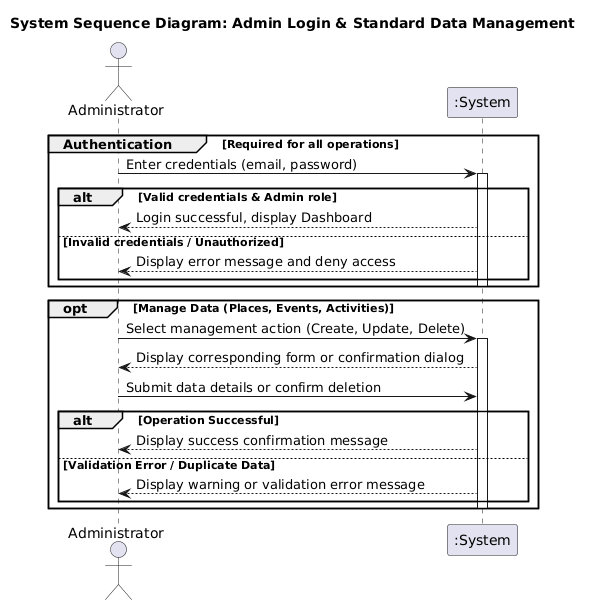
\includegraphics[width=0.85\textwidth,keepaspectratio]{images/diagram-ssd-admin-login.png}
\caption{System Sequence Diagram: การเข้าสู่ระบบและจัดการข้อมูลมาตรฐาน}
\label{fig:ssd_admin}
\end{figure}

\begin{figure}[H]
\centering
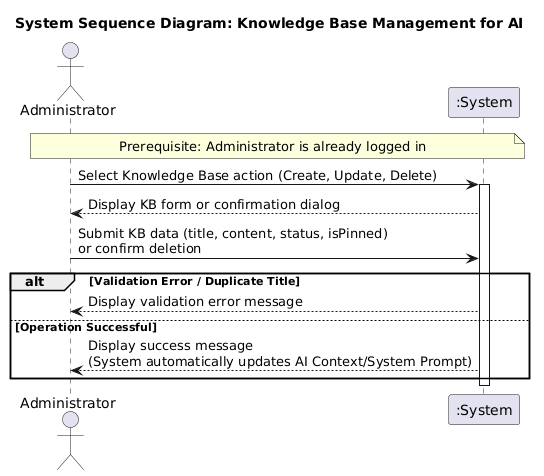
\includegraphics[width=0.85\textwidth,keepaspectratio]{images/diagram-ssd-admin-kb.png}
\caption{System Sequence Diagram: การจัดการฐานความรู้ (Knowledge Base)}
\label{fig:ssd_admin_kb}
\end{figure}

การจัดการข้อมูลแบบมาตรฐาน: ผู้ใช้งานส่งคำขอเข้าสู่ระบบ ระบบตรวจสอบความถูกต้องของข้อมูลบัญชี หากถูกต้องระบบอนุญาตให้เข้าถึงฟังก์ชัน CRUD โดยแต่ละคำสั่งระบบจะติดต่อกับฐานข้อมูลและส่งผลลัพธ์กลับ

การจัดการฐานความรู้: ผู้ดูแลระบบเลือกคำสั่ง (Create/Update/Delete) ระบบแสดงฟอร์มหรือกล่องยืนยัน เมื่อส่งข้อมูลแล้วระบบตรวจสอบภายใต้เงื่อนไขทางเลือก -- หากไม่ผ่านการตรวจสอบหรือหัวข้อซ้ำซ้อน ระบบแจ้งข้อผิดพลาด หากผ่านเกณฑ์ ระบบยืนยันความสำเร็จและปรับปรุงบริบทข้อมูล (System Prompt) ของ AI โดยอัตโนมัติ

\subsubsection{สำหรับระบบสะสมคะแนน (Point System)}

ระบบสะสมคะแนนมีลักษณะแตกต่างจากฟังก์ชันอื่นตรงที่ผู้ใช้งานที่เกี่ยวข้องสลับบทบาทกันระหว่างสองช่วง คือ นักท่องเที่ยว (Tourist) เป็นผู้ปฏิสัมพันธ์กับระบบโดยตรงในช่วงสะสมคะแนน ขณะที่ผู้ดูแลระบบ -- เจ้าหน้าที่ ททท. ขอนแก่น (Administrator) เป็นผู้ปฏิสัมพันธ์กับระบบแทนนักท่องเที่ยวในช่วงแลกของรางวัล จึงแยกแผนภาพออกเป็น 2 ส่วนตามลำดับ

\begin{figure}[H]
\centering
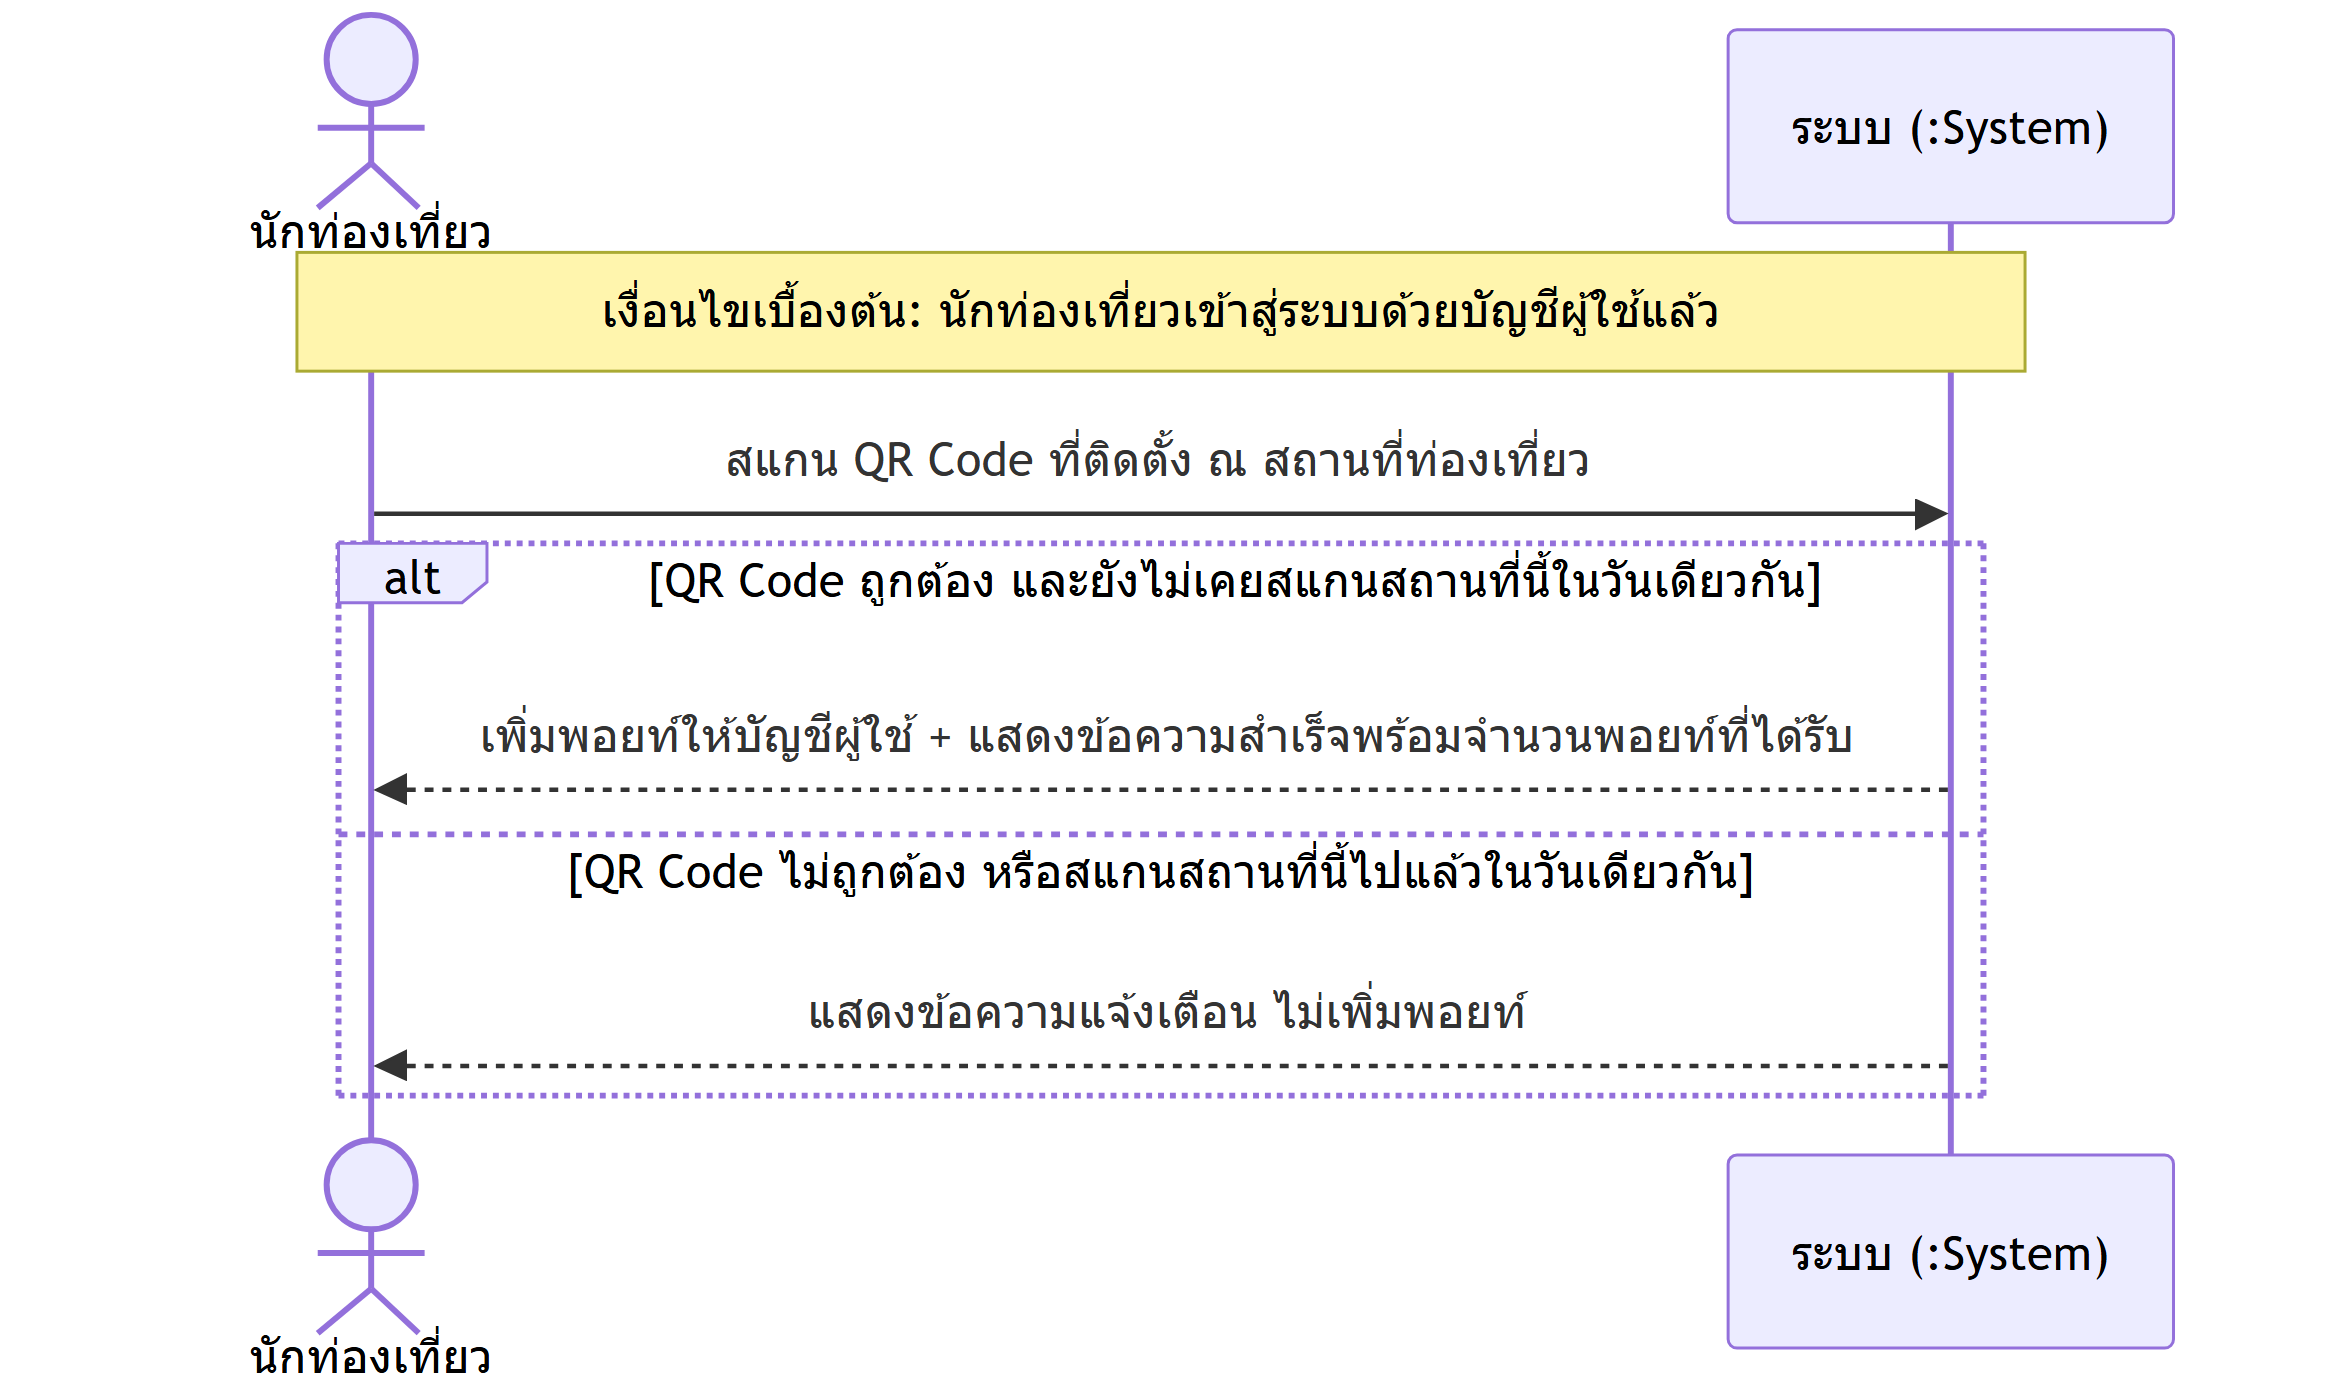
\includegraphics[width=0.85\textwidth,keepaspectratio]{images/diagram-ssd-point-scan.png}
\caption{System Sequence Diagram: สแกน QR สะสมพอยท์}
\label{fig:ssd_point_scan}
\end{figure}

\textbf{ฟังก์ชันสแกน QR Code สะสมพอยท์:} นักท่องเที่ยวที่เข้าสู่ระบบแล้วสแกน QR Code ที่ติดตั้งอยู่ ณ สถานที่ท่องเที่ยวที่เข้าร่วมโครงการ ภายใต้เงื่อนไขทางเลือก 2 กรณี คือ (1) QR Code ถูกต้องและยังไม่เคยสะสมพอยท์จากสถานที่นี้ในวันเดียวกัน ระบบเพิ่มพอยท์ให้บัญชีผู้ใช้และแสดงข้อความสำเร็จพร้อมจำนวนพอยท์ที่ได้รับ หรือ (2) QR Code ไม่ถูกต้อง หรือสะสมพอยท์จากสถานที่นี้ไปแล้วในวันเดียวกัน ระบบแสดงข้อความแจ้งเตือนโดยไม่เพิ่มพอยท์ (ดู UC-03; รายละเอียดการทำงานภายในระบบแสดงในภาพที่ \ref{fig:sequence_point_scan} หัวข้อ Sequence Diagram)

\begin{figure}[H]
\centering
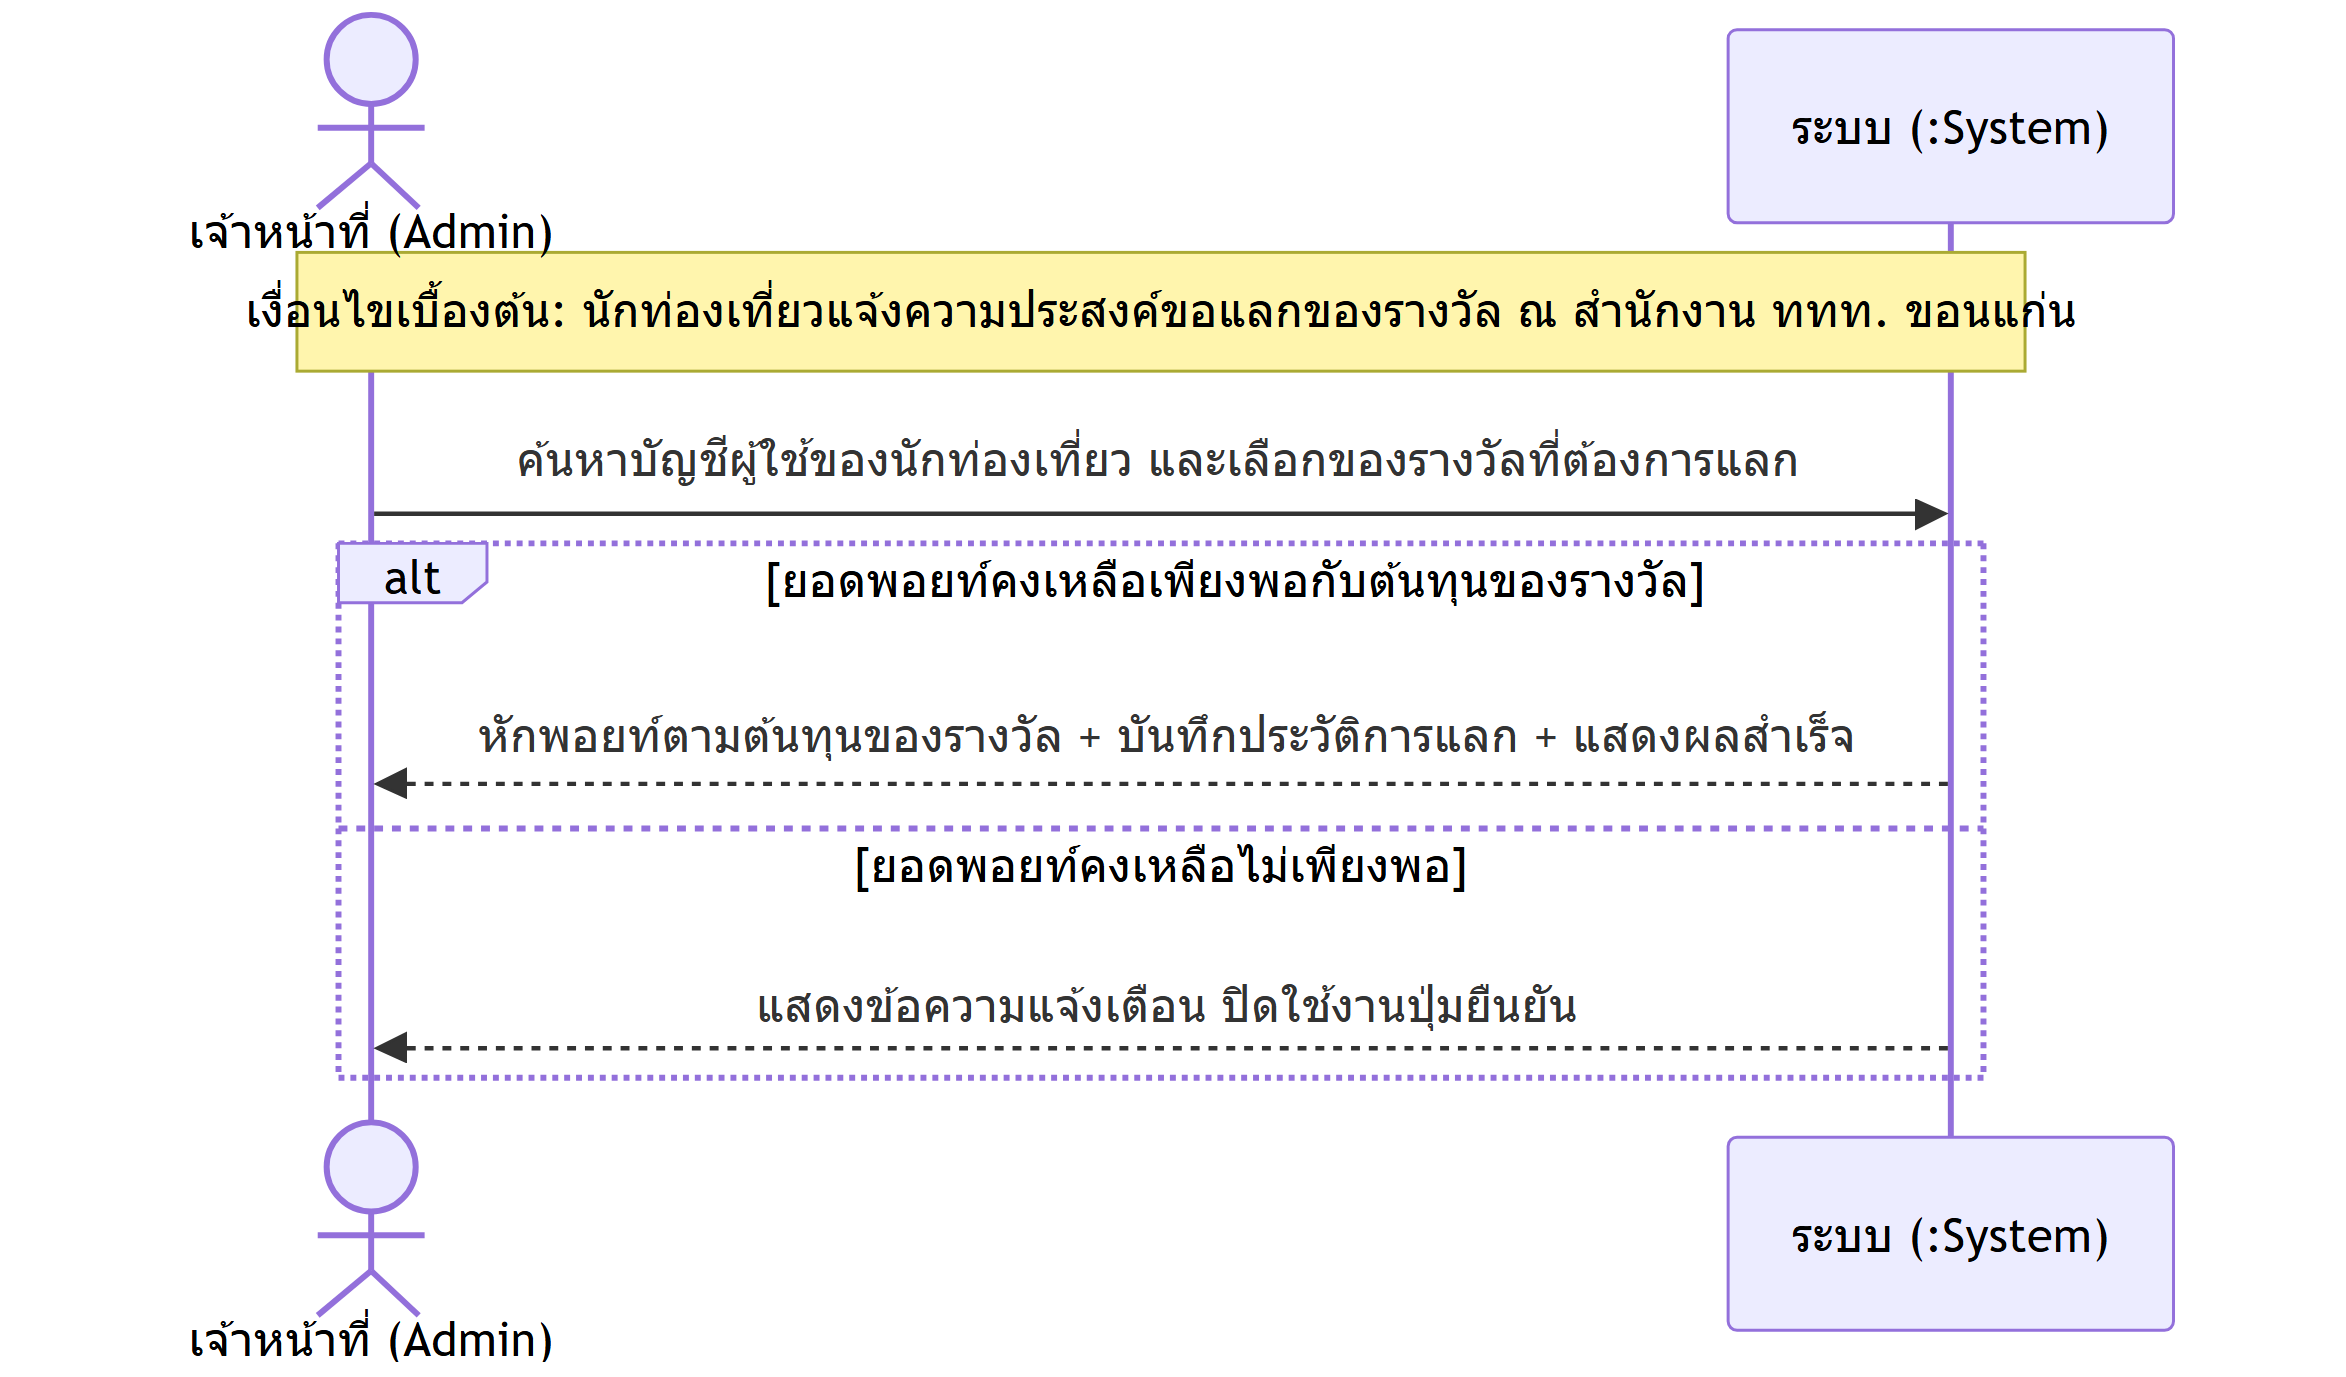
\includegraphics[width=0.85\textwidth,keepaspectratio]{images/diagram-ssd-point-redeem.png}
\caption{System Sequence Diagram: แลกของรางวัล ณ สำนักงาน ททท. ขอนแก่น}
\label{fig:ssd_point_redeem}
\end{figure}

\textbf{ฟังก์ชันแลกของรางวัล (Redemption):} เมื่อนักท่องเที่ยวเดินทางมาถึงสำนักงาน ททท. ขอนแก่นและแจ้งความประสงค์ขอแลกของรางวัลกับเจ้าหน้าที่ เจ้าหน้าที่ค้นหาบัญชีผู้ใช้ของนักท่องเที่ยวและเลือกของรางวัลที่ต้องการแลกในระบบ ภายใต้เงื่อนไขทางเลือก 2 กรณี คือ (1) ยอดพอยท์คงเหลือเพียงพอกับต้นทุนของรางวัล ระบบหักพอยท์ตามต้นทุนของรางวัล บันทึกประวัติการแลก และแสดงผลสำเร็จ หรือ (2) ยอดพอยท์คงเหลือไม่เพียงพอ ระบบแสดงข้อความแจ้งเตือนและปิดใช้งานปุ่มยืนยัน (ดู UC-08; รายละเอียดการทำงานภายในระบบแสดงในภาพที่ \ref{fig:sequence_point_redeem} หัวข้อ Sequence Diagram)

\subsection{แผนภาพกิจกรรม (Activity Diagram)}

ก่อนอธิบายการรับส่งข้อมูลระหว่าง Component ย่อย โครงงานนี้ได้จำลองตรรกะการตัดสินใจของอัลกอริทึมในการสร้างแผนการเดินทาง (Trip Planning Algorithm) เพื่อแสดงกระบวนการทำงานแบบเป็นลำดับขั้นตอน ตั้งแต่การรับเงื่อนไขจากผู้ใช้ การประมวลผล RAG การส่งคำสั่งให้ LLM ไปจนถึงการจัดการข้อมูลหลังการประมวลผล (Post-processing)

\begin{figure}[H]
\centering
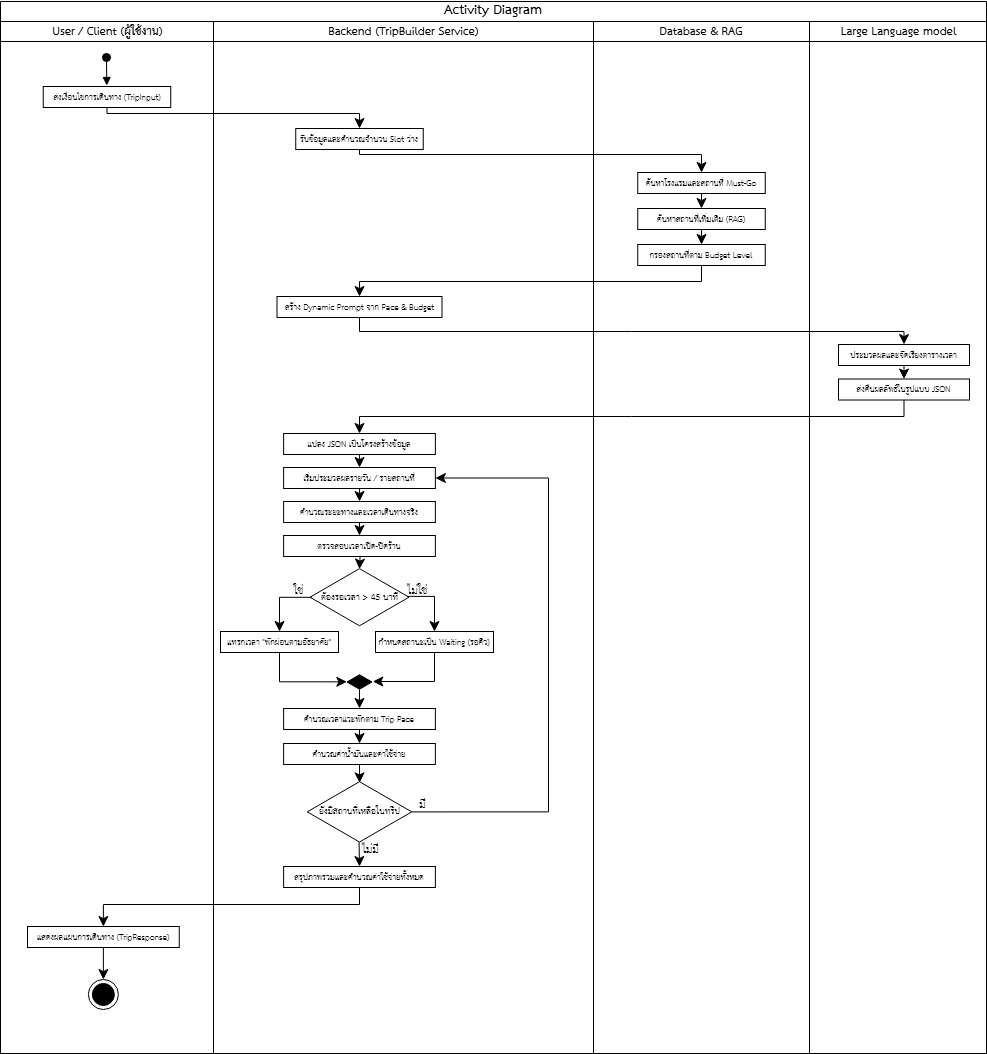
\includegraphics[width=0.9\textwidth,keepaspectratio]{images/diagram-activity.png}
\caption{Activity Diagram ตรรกะการประมวลผลเพื่อสร้างแผนการเดินทาง}
\label{fig:activity_diagram}
\end{figure}

แผนภาพใช้รูปแบบการแบ่งช่อง (Swimlane) แสดงขอบเขตความรับผิดชอบของ 4 องค์ประกอบหลัก ได้แก่ ผู้ใช้งาน (User/Client), ระบบหลังบ้าน (Backend: TripBuilder Service), ฐานข้อมูลและการดึงข้อมูล (Database \& RAG), และโมเดลภาษาขนาดใหญ่ (LLM) โดยมีขั้นตอนดังนี้ (1) ผู้ใช้งานส่งเงื่อนไขการเดินทาง (TripInput) เข้าสู่ระบบ (2) ระบบหลังบ้านคำนวณช่องว่าง (Slot) ของเวลาในทริป ค้นหาโรงแรม สถานที่บังคับ (Must-Go) และใช้ RAG ค้นหาสถานที่เพิ่มเติมตามความสนใจ พร้อมกรองตามระดับงบประมาณ (3) ระบบสร้าง Dynamic Prompt จากความเร็วทริป (Pace) และงบประมาณ ส่งให้ LLM ประมวลผลและจัดเรียงตารางเวลาเบื้องต้น คืนผลลัพธ์เป็น JSON (4) ระบบหลังบ้านแปลงข้อมูล JSON และวนลูปตรวจสอบทีละสถานที่ในแต่ละวัน คำนวณระยะทางและเวลาเดินทางจริง ตรวจสอบเวลาเปิด-ปิด (หากต้องรอเปิดนานกว่า 45 นาที แทรกกิจกรรม ``พักผ่อนตามอัธยาศัย'' หากรอน้อยกว่ากำหนดสถานะ ``Waiting'') คำนวณเวลาแวะพักตามลักษณะทริปและค่าน้ำมัน (5) ระบบวนลูปจนครบทุกสถานที่ สรุปภาพรวมและค่าใช้จ่ายทั้งหมด พร้อมส่งผลลัพธ์ (TripResponse) กลับไปแสดงผลให้ผู้ใช้งานทราบ

% -----------------------------------------------------------
\section{การออกแบบระบบ}
% -----------------------------------------------------------

\subsection{สถาปัตยกรรมของระบบ}

แนวคิดการออกแบบระบบถูกพัฒนาภายใต้สถาปัตยกรรมไมโครเซอร์วิส เพื่อแยกส่วนการทำงานออกจากกันอย่างชัดเจน ทั้งในเชิงตรรกะ (Logical) และเชิงกายภาพ (Physical) ทำให้แอปพลิเคชันสามารถรองรับการขยายตัว (Scalability) ได้ดี

\begin{figure}[H]
\centering
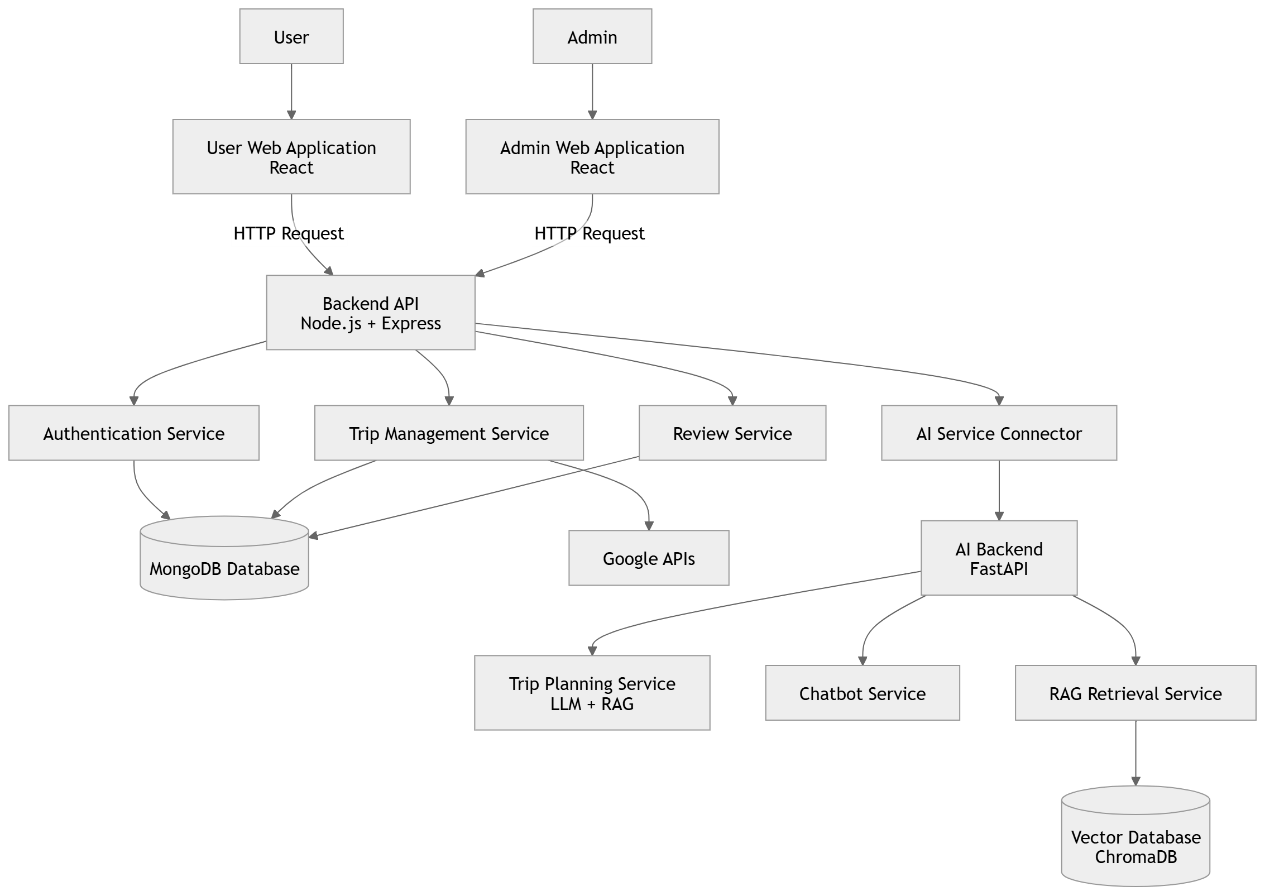
\includegraphics[width=0.85\textwidth,keepaspectratio]{images/diagram-architecture.png}
\caption{สถาปัตยกรรมของระบบ}
\label{fig:architecture}
\end{figure}

\textit{หมายเหตุ: ภาพที่ \ref{fig:architecture} เป็นแผนภาพร่างตั้งต้นของโครงงาน ซึ่งมีรายละเอียดบางส่วนคลาดเคลื่อนจากสถาปัตยกรรมที่อธิบายไว้ด้านล่างนี้ (เช่น ไม่มี Mobile Application, ไม่มี API Gateway แยก, ฐานข้อมูลไม่ใช่ MongoDB) -- ให้ยึดคำอธิบายด้านล่างนี้เป็นหลัก}

\begin{enumerate}
\item \textbf{ส่วนติดต่อผู้ใช้งาน (Frontend Component):} พัฒนาด้วย React ร่วมกับ Vite และ react-router-dom เป็นเว็บแอปพลิเคชัน (Web Application) เพียงชุดเดียว ให้บริการทั้งฝั่งผู้ใช้งานทั่วไป (Tourist) และส่วน Admin Portal ภายใต้เส้นทาง (Route) เดียวกัน ยังไม่มีการแยกพัฒนาเป็น Mobile Application ต่างหาก
\item \textbf{ส่วนการจัดการระบบหลัก (Core Backend Component):} ใช้ Node.js (Express) ทำหน้าที่เป็น REST API ให้บริการ CRUD ข้อมูลสถานที่ กิจกรรม ฐานความรู้ QR และของรางวัล โดยเชื่อมต่อฐานข้อมูล PostgreSQL ผ่าน Supabase (บริการ PostgreSQL ที่มีการจัดการให้ -- Managed Service) ด้วยไลบรารี @supabase/supabase-js ส่วนนี้ไม่ได้ทำหน้าที่เป็น API Gateway ให้ AI Service -- Frontend เรียก AI Service (chatbot-service) โดยตรงเป็นอีกบริการหนึ่งแยกจากกัน และมีสคริปต์ Data Pipeline แยกต่างหาก (backend/scripts) สำหรับดึงและนำเข้าข้อมูลจาก Google Places API
\item \textbf{ส่วนบริการปัญญาประดิษฐ์ (AI Service):} พัฒนาด้วย Python (FastAPI) เป็นบริการอิสระ (chatbot-service) ที่ Frontend เรียกใช้งานโดยตรง ทำหน้าที่ประมวลผล RAG, แชตบอต และ Trip Planner โดยเรียกใช้โมเดลภาษาขนาดใหญ่ (Google Gemini รุ่น gemini-2.5-flash/gemini-2.5-pro) ผ่าน API Gateway ของมหาวิทยาลัยขอนแก่นที่มีรูปแบบ Request/Response แบบเดียวกับ OpenAI API (ไม่ได้ใช้ Ollama หรือรันโมเดลภายในเครื่อง) และค้นคืนข้อมูล (Retrieval) จาก Vector Database ซึ่งไม่ได้แยกเป็นฐานข้อมูลต่างหาก (ไม่ใช่ Chroma) แต่ใช้ส่วนขยาย pgvector ที่ติดตั้งอยู่ในฐานข้อมูล PostgreSQL ตัวเดียวกับที่ Core Backend ใช้ (คอลัมน์ embedding ในตาราง places และ knowledge\_base) โดยแปลงข้อความเป็นเวกเตอร์ด้วยโมเดล sentence-transformers (paraphrase-multilingual-MiniLM-L12-v2) ที่รันในเครื่องของบริการเอง ไม่ได้เรียกผ่าน API ภายนอก
\end{enumerate}

\subsection{Sequence Diagram}

\begin{figure}[H]
\centering
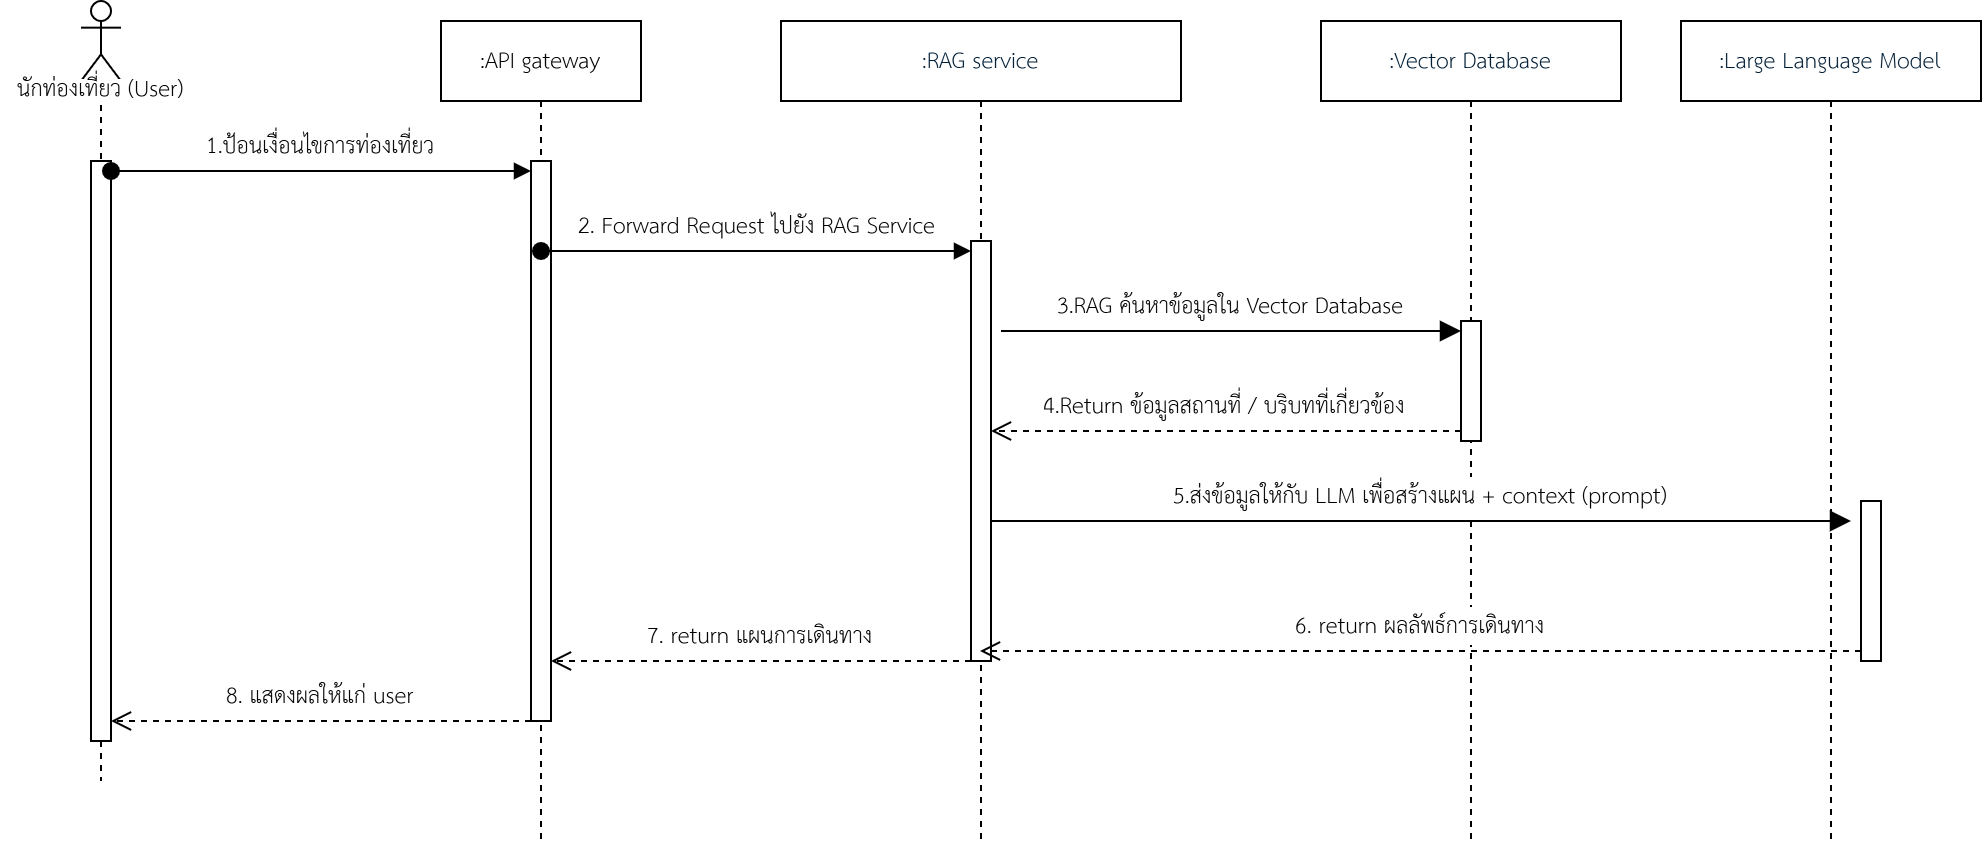
\includegraphics[width=0.85\textwidth,keepaspectratio]{images/diagram-sequence-trip.png}
\caption{Detailed Sequence Diagram: การสร้างแผนการเดินทางด้วย RAG และ LLM}
\label{fig:sequence_user}
\end{figure}

\textbf{การสร้างแผนการเดินทางด้วย RAG และ LLM} ประกอบด้วย 4 ส่วนหลัก ได้แก่ นักท่องเที่ยว (Frontend), Trip Planner Service (chatbot-service), ฐานข้อมูล PostgreSQL/pgvector (Vector Search) และ LLM มีลำดับขั้นตอนโดยสรุป: (1) Frontend ส่งคำขอเงื่อนไขการเดินทางไปยัง Trip Planner Service โดยตรง (2) Trip Planner Service ค้นหาสถานที่ที่สอดคล้องกับความสนใจในตาราง places ผ่านฟังก์ชัน match\_places (Vector Similarity ด้วย pgvector) พร้อมกรองตามงบประมาณและขอบเขตพื้นที่ (3) ฐานข้อมูลคืนค่ารายชื่อสถานที่ที่เกี่ยวข้อง (4) Trip Planner Service ประกอบ Prompt จากสถานที่ที่ได้และเงื่อนไขผู้ใช้ ส่งให้ LLM สร้างตารางเวลาเบื้องต้น (5) LLM ส่งผลลัพธ์กลับเป็น JSON (6) Trip Planner Service ตรวจสอบคุณภาพแผนด้วย LLM-as-a-Judge และคำนวณระยะทาง/เวลา/สถานะเปิด-ปิดจริงเพิ่มเติม (Post-processing) (7) Trip Planner Service ส่งแผนที่สมบูรณ์กลับไปยัง Frontend โดยตรงเพื่อแสดงผล

\textbf{การทำงานของระบบผู้ช่วยเสมือน (แชตบอต)} มีลำดับเหตุการณ์โดยสรุป: Frontend ส่งคำถามไปยัง แชตบอต Service (chatbot-service) โดยตรง $\rightarrow$ แชตบอต Service ค้นหาบริบทที่เกี่ยวข้องในตาราง places/knowledge\_base ผ่าน pgvector (Vector Similarity Search) $\rightarrow$ ดึงข้อมูลสถานที่/ความรู้ที่เกี่ยวข้องมากที่สุด $\rightarrow$ ประกอบคำสั่ง (System Prompt + Context ที่ค้นได้ + ประวัติการสนทนา + ข้อความผู้ใช้) $\rightarrow$ ส่งให้ LLM ประมวลผลแบบ Streaming $\rightarrow$ LLM ทยอยส่งคำตอบกลับ $\rightarrow$ แชตบอต Service ส่งต่อคำตอบแบบ Streaming ไปยัง Frontend $\rightarrow$ แสดงผลบนหน้าจอผู้ใช้แบบทยอยปรากฏ (Streaming Response)

\begin{figure}[H]
\centering
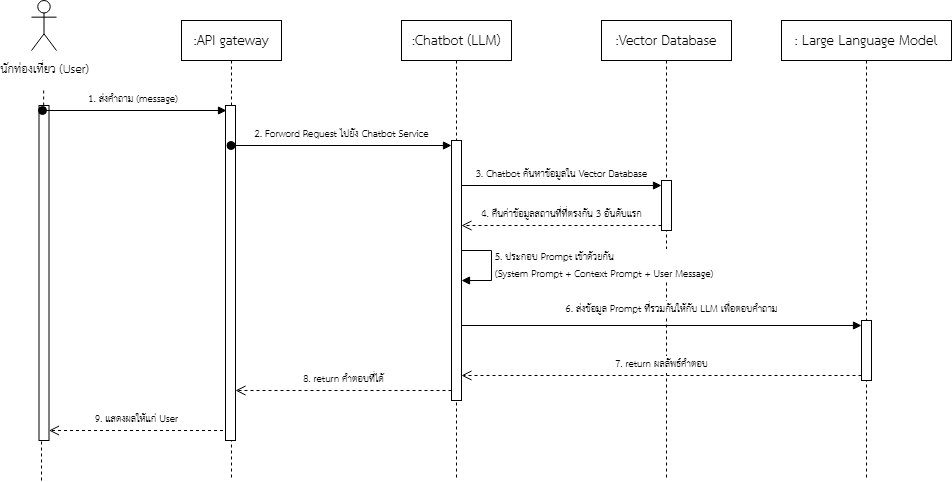
\includegraphics[width=0.85\textwidth,keepaspectratio]{images/diagram-sequence-chatbot.png}
\caption{Detailed Sequence Diagram: การทำงานของระบบผู้ช่วยเสมือน (แชตบอต)}
\label{fig:sequence_chatbot}
\end{figure}

\begin{figure}[H]
\centering
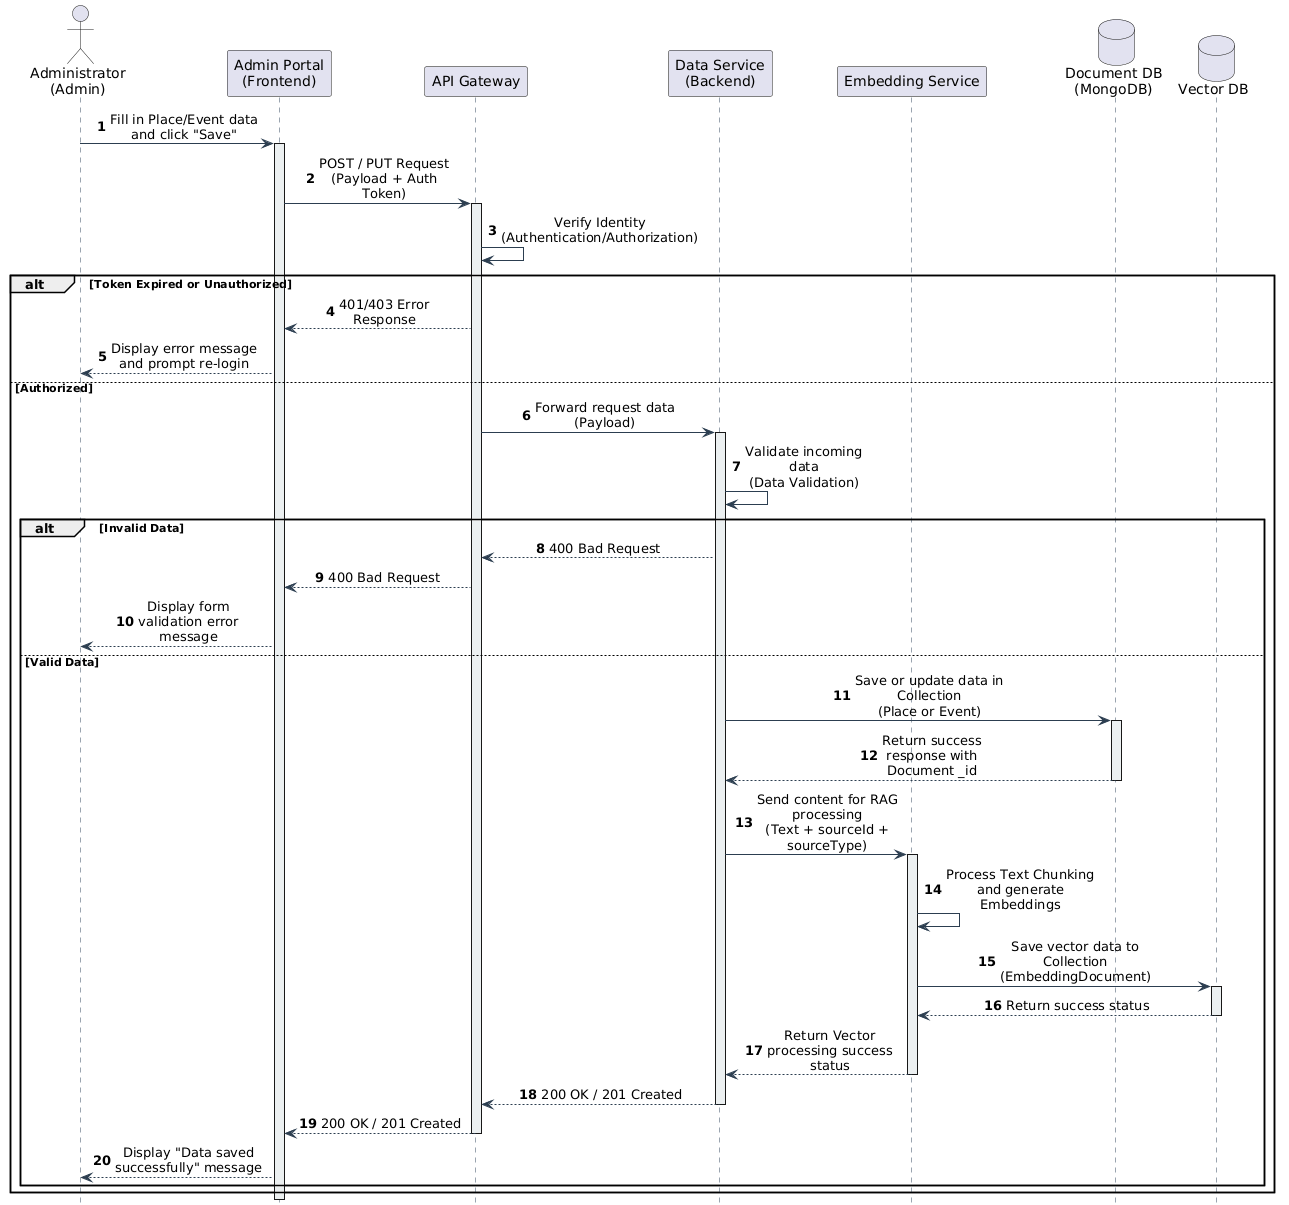
\includegraphics[width=0.85\textwidth,keepaspectratio]{images/diagram-sequence-admin-data.png}
\caption{Detailed Sequence Diagram สำหรับผู้ดูแลระบบ}
\label{fig:sequence_admin}
\end{figure}

การจัดการข้อมูล (สถานที่/กิจกรรม/ฐานความรู้/QR/ของรางวัล) ทำผ่าน Core Backend (Node.js/Express) โดยตรง กระบวนการเริ่มจากผู้ดูแลระบบส่งคำขอจาก Admin Portal ไปยัง Backend ซึ่งบันทึก/ปรับปรุงข้อมูลลงตารางที่เกี่ยวข้องในฐานข้อมูล PostgreSQL (Supabase) แล้วส่งผลลัพธ์กลับไปยังส่วนติดต่อผู้ใช้ในรูปแบบสถานะสำเร็จ การอัปเดตค่า Embedding ที่เกี่ยวข้องดำเนินการตามที่ระบุในหัวข้อการติดต่อกับฐานข้อมูลและ Services

\begin{figure}[H]
\centering
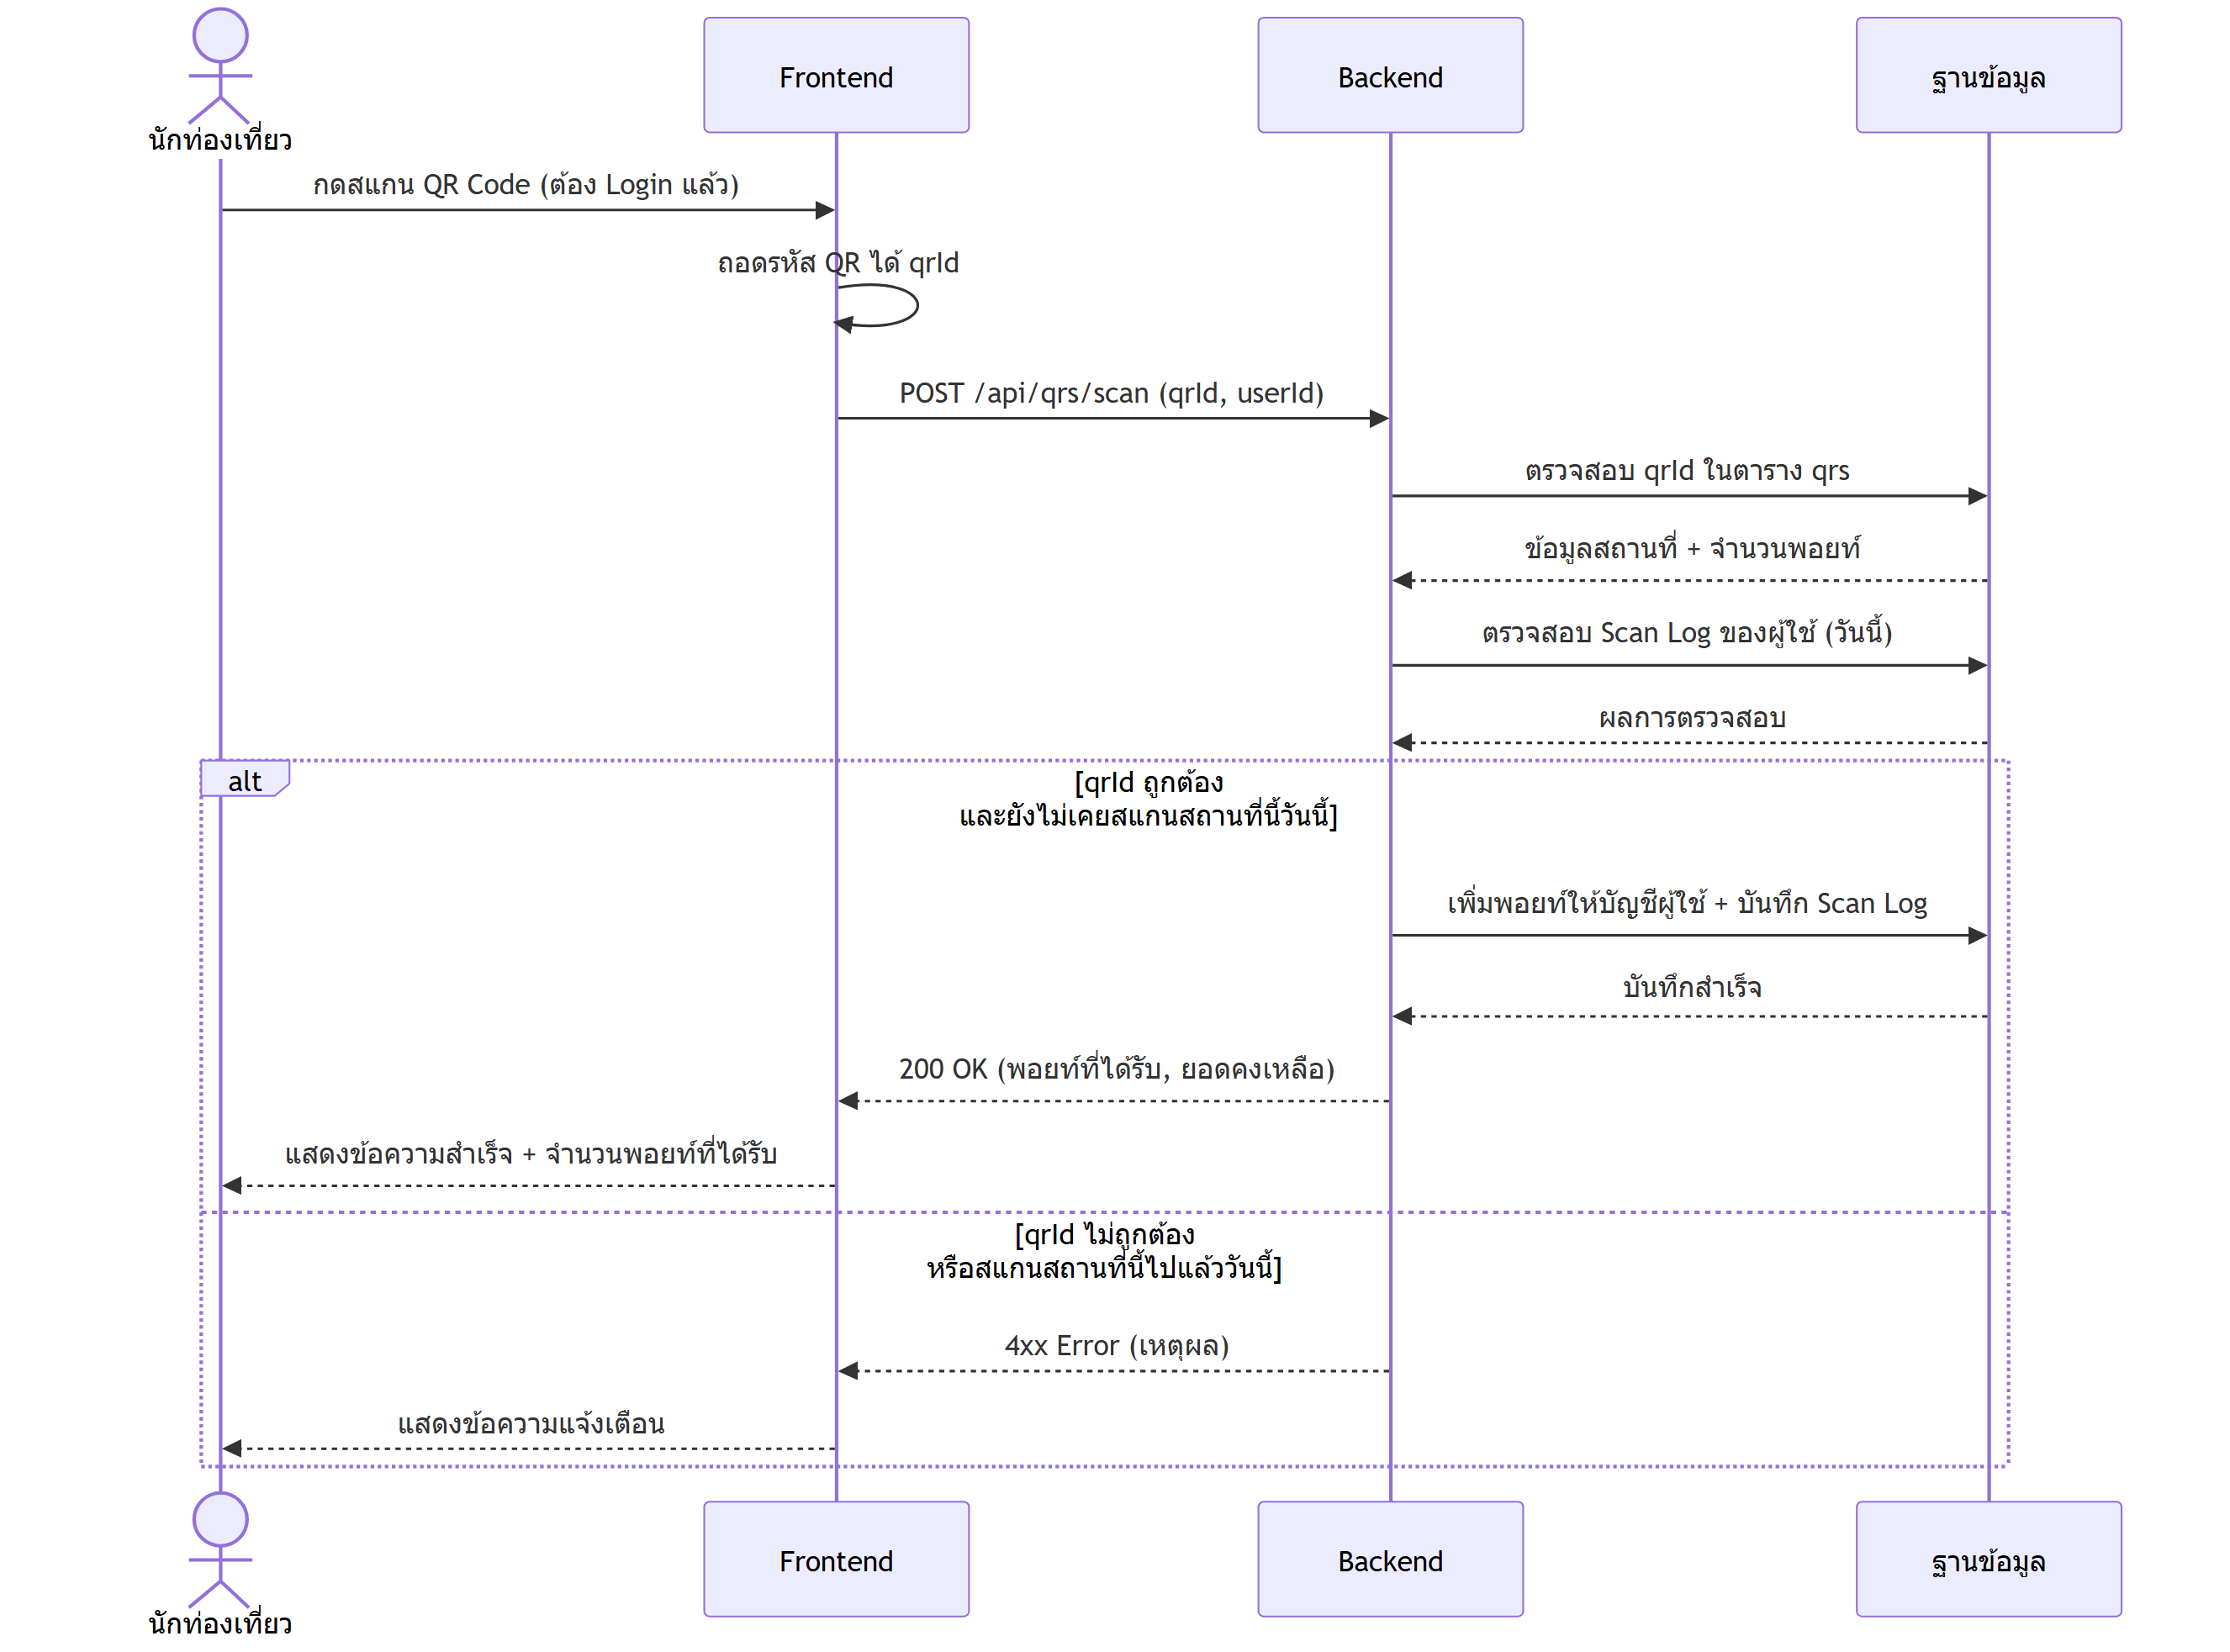
\includegraphics[width=0.85\textwidth,keepaspectratio]{images/diagram-sequence-point-scan.png}
\caption{Detailed Sequence Diagram: สแกน QR สะสมพอยท์}
\label{fig:sequence_point_scan}
\end{figure}

\textbf{ฟังก์ชันสแกน QR Code สะสมพอยท์} ประกอบด้วย 3 ส่วนหลัก ได้แก่ นักท่องเที่ยว (Frontend), Backend และฐานข้อมูล มีลำดับขั้นตอนโดยสรุป: (1) นักท่องเที่ยวกดสแกน QR Code ผ่านกล้องของอุปกรณ์ Frontend ถอดรหัสอ้างอิง (qrId) จาก QR Code (2) Frontend ส่ง qrId พร้อมข้อมูลบัญชีผู้ใช้ไปยัง Backend ผ่าน API (3) Backend ตรวจสอบว่า qrId มีอยู่จริงในตาราง qrs และดึงจำนวนพอยท์ที่กำหนดไว้กับสถานที่นั้น (4) Backend ตรวจสอบ Scan Log ของผู้ใช้ว่าเคยสะสมพอยท์จากสถานที่เดียวกันในวันเดียวกันแล้วหรือไม่ (Rate Limiting) (5) หากผ่านทั้งสองเงื่อนไข Backend เพิ่มพอยท์ให้บัญชีผู้ใช้และบันทึก Scan Log ลงฐานข้อมูล แล้วตอบกลับ Frontend ด้วยจำนวนพอยท์ที่ได้รับ หากไม่ผ่านเงื่อนไขใดเงื่อนไขหนึ่ง Backend ตอบกลับด้วยข้อผิดพลาดพร้อมเหตุผลโดยไม่แก้ไขข้อมูลใด ๆ

\begin{figure}[H]
\centering
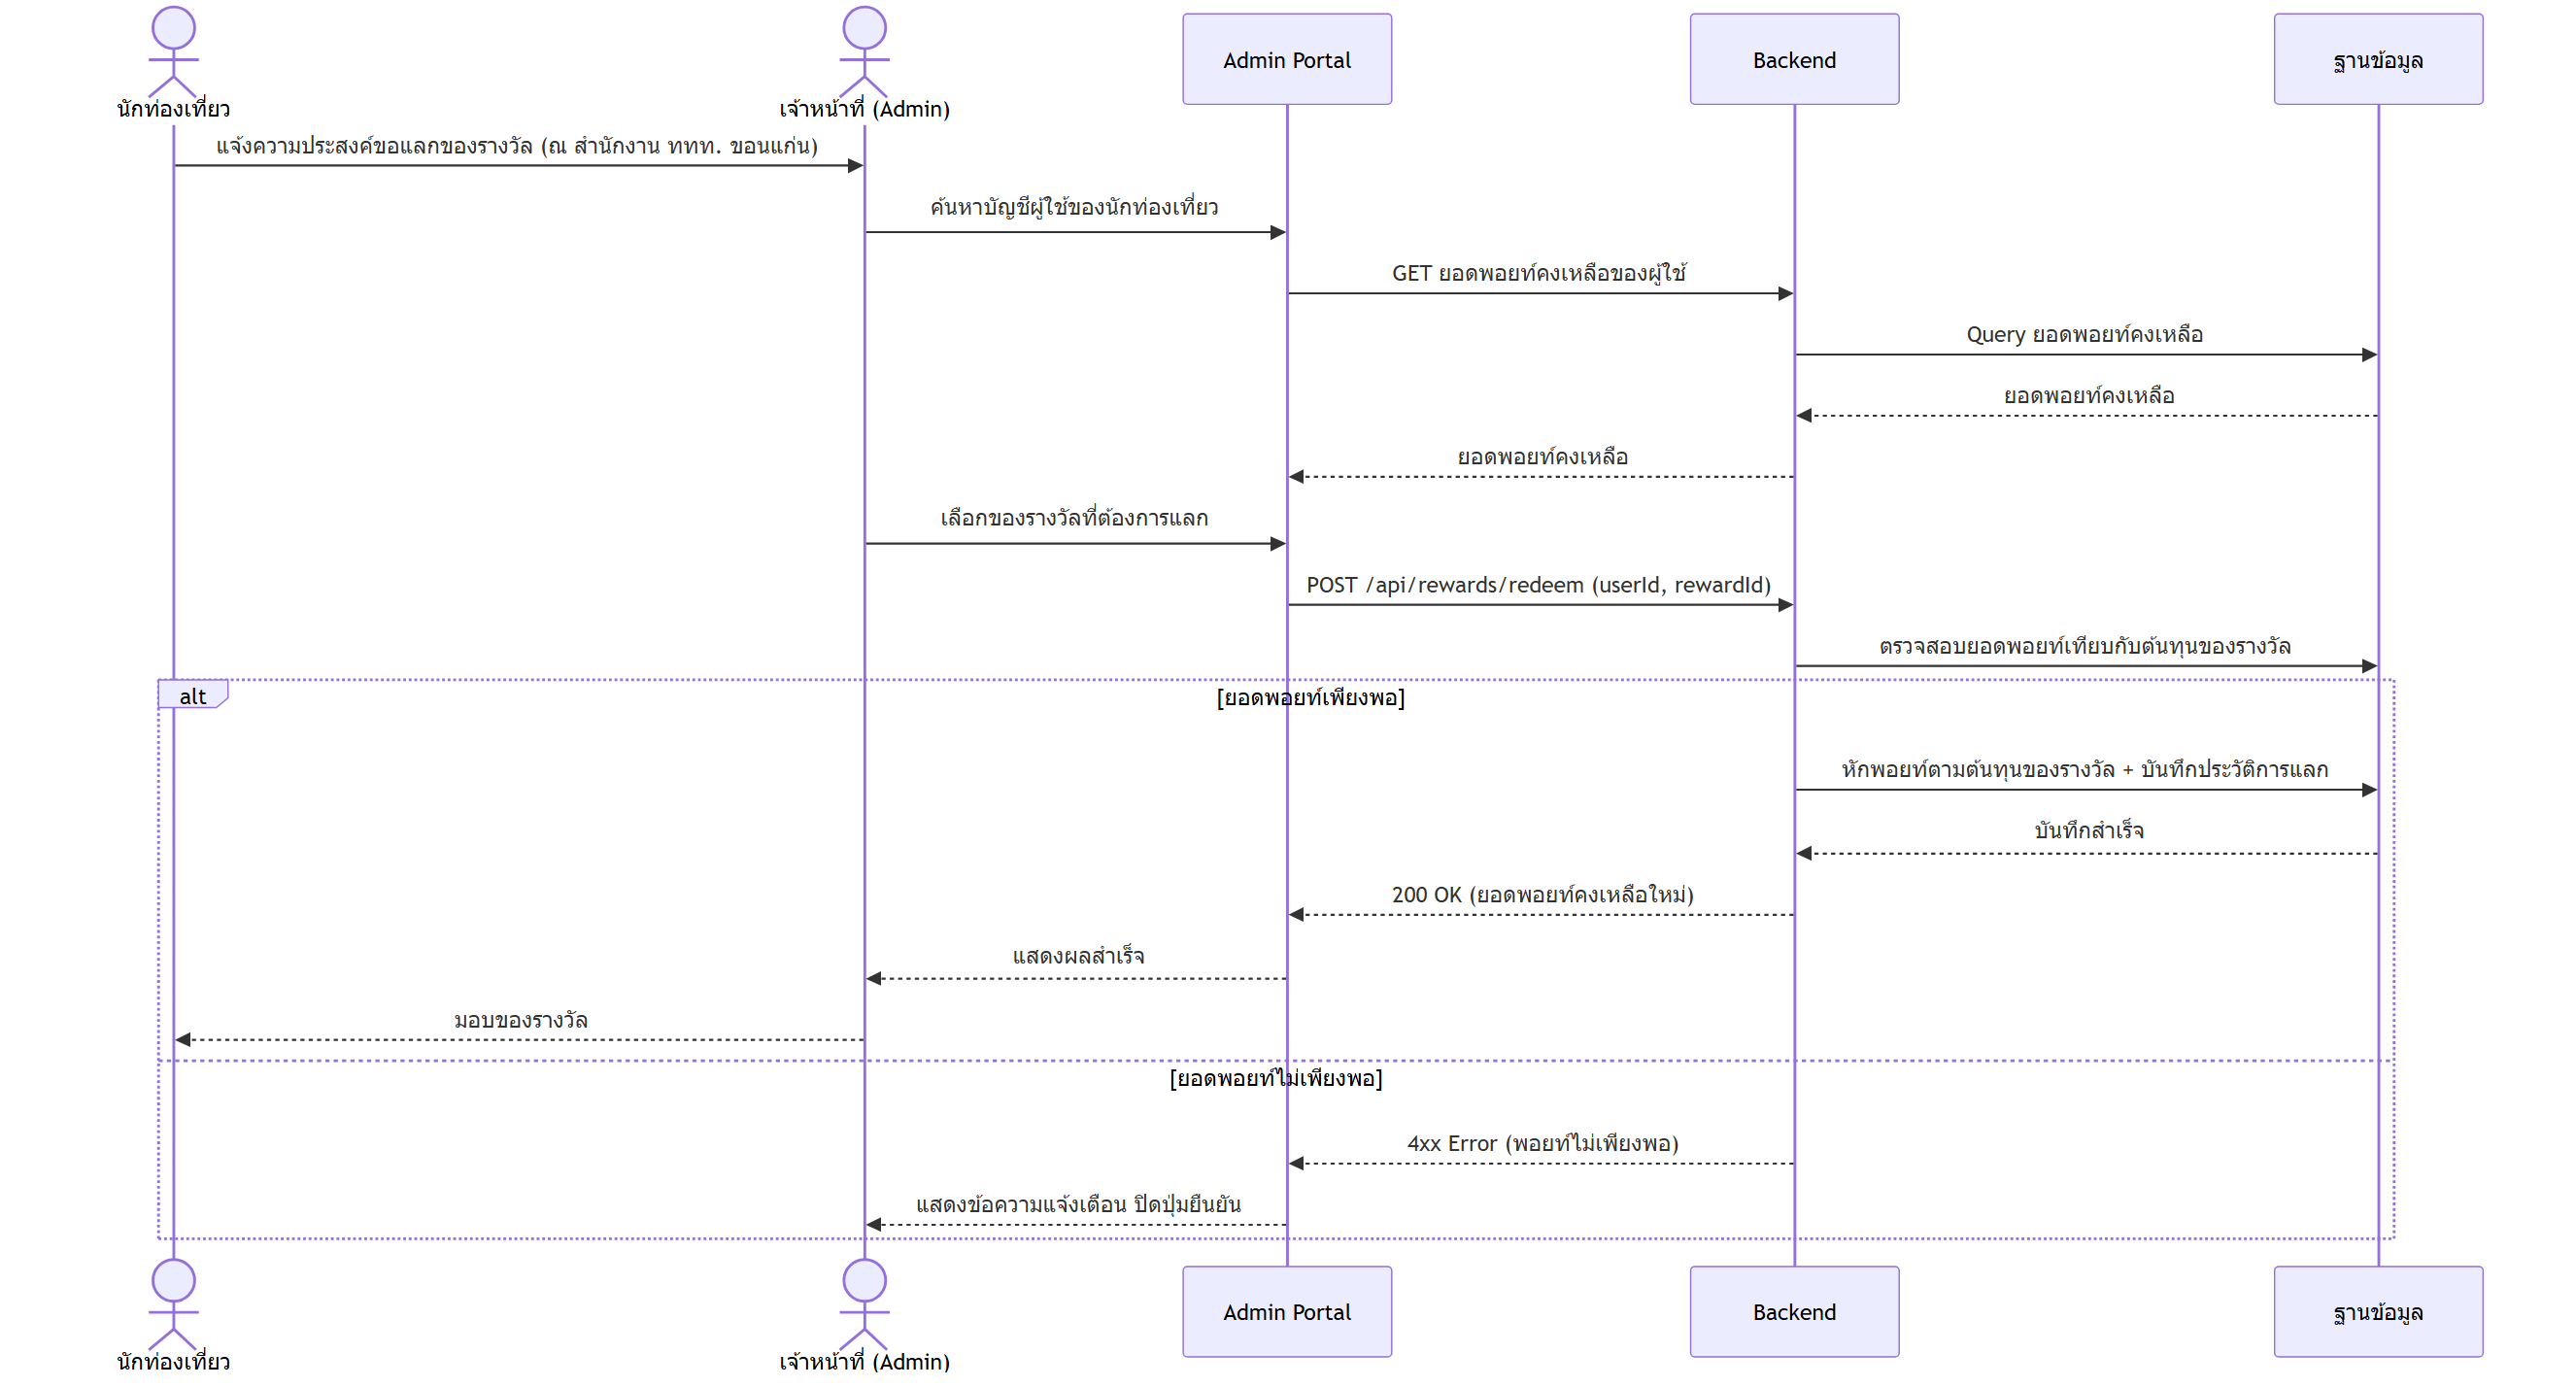
\includegraphics[width=0.85\textwidth,keepaspectratio]{images/diagram-sequence-point-redeem.png}
\caption{Detailed Sequence Diagram: แลกของรางวัล ณ สำนักงาน ททท. ขอนแก่น}
\label{fig:sequence_point_redeem}
\end{figure}

\textbf{ฟังก์ชันแลกของรางวัล (Redemption)} ประกอบด้วย 4 ส่วนหลัก ได้แก่ เจ้าหน้าที่ (Admin Portal), Backend, ฐานข้อมูล และนักท่องเที่ยวในฐานะผู้รับผลประโยชน์นอกระบบ มีลำดับขั้นตอนโดยสรุป: (1) เจ้าหน้าที่ค้นหาบัญชีผู้ใช้ของนักท่องเที่ยวใน Admin Portal ซึ่งเรียก Backend เพื่อดึงยอดพอยท์คงเหลือจากฐานข้อมูล (2) เจ้าหน้าที่เลือกของรางวัลที่นักท่องเที่ยวต้องการแลก Admin Portal ส่งคำขอแลกของรางวัลไปยัง Backend (3) Backend ตรวจสอบยอดพอยท์คงเหลือเทียบกับต้นทุนของรางวัลในฐานข้อมูล (4) หากยอดพอยท์เพียงพอ Backend หักพอยท์ตามต้นทุนของรางวัลและบันทึกประวัติการแลก (ผู้ใช้งาน, รางวัล, เจ้าหน้าที่ผู้ดำเนินการ, เวลา) ลงฐานข้อมูล แล้วตอบกลับ Admin Portal ด้วยยอดพอยท์คงเหลือใหม่ให้เจ้าหน้าที่มอบของรางวัลแก่นักท่องเที่ยว หากยอดพอยท์ไม่เพียงพอ Backend ตอบกลับด้วยข้อผิดพลาดโดยไม่แก้ไขข้อมูลใด ๆ

\subsection{การออกแบบฐานข้อมูล}

ระบบใช้ฐานข้อมูลเชิงสัมพันธ์ (Relational Database) ด้วย PostgreSQL ผ่านบริการ Supabase เป็นฐานข้อมูลหลักเพียงฐานเดียว โดยติดตั้งส่วนขยาย pgvector เพิ่มเติมเพื่อให้คอลัมน์ embedding ในตาราง places และ knowledge\_base จัดเก็บเวกเตอร์ฝังตัว (Embedding Vectors) ที่ใช้ในกระบวนการค้นคืนข้อมูลเชิงความหมาย (Semantic Retrieval) ได้โดยตรง จึงไม่มีฐานข้อมูลเวกเตอร์แยกต่างหาก ข้อมูลกึ่งโครงสร้าง (Semi-Structured Data) ที่ได้จาก Google Places API ซึ่งไม่สามารถแตกเป็นคอลัมน์ตายตัวได้ทั้งหมด ถูกเก็บสำรองไว้ในคอลัมน์ประเภท jsonb (raw\_data) เพื่อความยืดหยุ่น

ความสัมพันธ์ระหว่างตารางแสดงดังภาพที่ \ref{fig:erd} โดยเขียนตามสัญกรณ์ Chen (Chen Notation) ในระดับแนวคิด (Conceptual Level) -- สี่เหลี่ยมผืนผ้าแทน Entity วงรีแทน Attribute (ขีดเส้นใต้คือ Primary Key) สี่เหลี่ยมข้าวหลามตัดแทนความสัมพันธ์ (Relationship) พร้อมกำกับ Cardinality แบบ (min, max) บนเส้นเชื่อมแต่ละด้าน และกรอบเส้นประ (knowledge\_base) คือ Entity อิสระที่ไม่มีความสัมพันธ์กับ Entity อื่น เพื่อความกระชับ ภาพนี้แสดงเฉพาะ Primary Key ของแต่ละ Entity เท่านั้น รายละเอียดคอลัมน์ทั้งหมดแสดงในตารางที่ \ref{tab:db_place}--\ref{tab:db_redemptions} ถัดไป

ความสัมพันธ์ ``สแกน'' (ระหว่าง users กับ qrs) และ ``แลก'' (ระหว่าง users กับ rewards) เป็นความสัมพันธ์แบบ กลุ่มต่อกลุ่ม (Many-to-Many) ที่มี Attribute ของตัวเอง (points\_earned/scanned\_at และ points\_spent/redeemed\_by/redeemed\_at ตามลำดับ) ซึ่งเมื่อแปลงเป็นฐานข้อมูลเชิงสัมพันธ์จริงจะกลายเป็นตาราง qr\_scans และ redemptions ตามลำดับ (ดูตารางที่ \ref{tab:db_qrscans}, \ref{tab:db_redemptions}) ส่วนความสัมพันธ์ ``จัดขึ้นที่'' ระหว่าง places กับ events เป็นความสัมพันธ์แบบ Optional -- events ด้านที่มี Cardinality (0,1) หมายความว่ากิจกรรมหนึ่งรายการอาจจะยังไม่ได้ผูกกับสถานที่ใดในตาราง places เลยก็ได้ (กรอกแค่ venue\_name/venue\_lat/venue\_lng เอง) แต่ถ้าสถานที่จัดงานนั้นมีอยู่แล้วในตาราง places ก็สามารถผูกไว้เพื่อให้แสดงรายการกิจกรรมที่จะเกิดขึ้น ณ สถานที่นั้นได้

\begin{figure}[H]
\centering
\resizebox{0.98\linewidth}{!}{%
\begin{tikzpicture}[
  entity/.style={draw, thick, rectangle, minimum width=2.5cm, minimum height=0.85cm, align=center, font=\small, inner sep=3pt},
  standalone/.style={draw, thick, rectangle, dashed, minimum width=2.5cm, minimum height=0.85cm, align=center, font=\small, inner sep=3pt},
  relationship/.style={draw, thick, diamond, minimum width=2.0cm, minimum height=1.3cm, align=center, font=\scriptsize, inner sep=1pt},
  attribute/.style={draw, thin, ellipse, align=center, font=\scriptsize, inner sep=2pt},
  edge/.style={thick},
  card/.style={font=\scriptsize, fill=white, inner sep=1pt},
  node distance=3.0cm and 4.4cm
]

% ---------- entities ----------
\node[entity] (users) {users};
\node[entity, below=of users] (qrs) {qrs};
\node[entity, below=of qrs] (places) {places};
\node[entity, below=of places] (events) {events};
\node[entity, right=of users] (rewards) {rewards};
\node[standalone, above right=1.4cm and 0.3cm of rewards] (kb) {knowledge\_base};

% ---------- relationships ----------
\node[relationship] (rel_scan) at ($(users)!0.5!(qrs)$) {สแกน};
\node[relationship] (rel_has) at ($(qrs)!0.5!(places)$) {มี};
\node[relationship] (rel_occurs) at ($(places)!0.5!(events)$) {จัดขึ้นที่};
\node[relationship] (rel_redeem) at ($(users)!0.5!(rewards)$) {แลก};

\draw[edge] (users) -- (rel_scan) -- (qrs);
\draw[edge] (qrs) -- (rel_has) -- (places);
\draw[edge] (places) -- (rel_occurs) -- (events);
\draw[edge] (users) -- (rel_redeem) -- (rewards);

% ---------- cardinalities ----------
\node[card] at ($(users)!0.3!(rel_scan)$) {(0,N)};
\node[card] at ($(rel_scan)!0.3!(qrs)$) {(0,N)};
\node[card] at ($(qrs)!0.3!(rel_has)$) {(1,1)};
\node[card] at ($(rel_has)!0.3!(places)$) {(1,N)};
\node[card] at ($(places)!0.3!(rel_occurs)$) {(0,N)};
\node[card] at ($(rel_occurs)!0.3!(events)$) {(0,1)};
\node[card] at ($(users)!0.3!(rel_redeem)$) {(0,N)};
\node[card] at ($(rel_redeem)!0.3!(rewards)$) {(0,N)};

% ---------- entity key attributes (PK) ----------
\node[attribute, left=0.9cm of users] (users_id) {\underline{id}};
\draw[thin] (users) -- (users_id);
\node[attribute, left=0.9cm of qrs] (qrs_id) {\underline{id}};
\draw[thin] (qrs) -- (qrs_id);
\node[attribute, left=0.9cm of places] (places_id) {\underline{id}};
\draw[thin] (places) -- (places_id);
\node[attribute, left=0.9cm of events] (events_id) {\underline{id}};
\draw[thin] (events) -- (events_id);
\node[attribute, above=0.7cm of rewards] (rewards_id) {\underline{id}};
\draw[thin] (rewards) -- (rewards_id);
\node[attribute, above=0.7cm of kb] (kb_id) {\underline{id}};
\draw[thin] (kb) -- (kb_id);

% ---------- relationship attributes ----------
% rel_scan: up/down taken by entity edges -> attributes go to the left (away from rel_redeem)
\node[attribute, above left=0.6cm and 0.6cm of rel_scan] (a_earned) {points\_earned};
\node[attribute, below left=0.6cm and 0.6cm of rel_scan] (a_scannedat) {scanned\_at};
\draw[thin] (rel_scan) -- (a_earned);
\draw[thin] (rel_scan) -- (a_scannedat);

% rel_redeem: left/right taken by entity edges -> attributes go up/down
\node[attribute, above left=1.0cm and 0.5cm of rel_redeem] (a_spent) {points\_spent};
\node[attribute, above right=1.0cm and 0.5cm of rel_redeem] (a_by) {redeemed\_by};
\node[attribute, below=1.0cm of rel_redeem] (a_redat) {redeemed\_at};
\draw[thin] (rel_redeem) -- (a_spent);
\draw[thin] (rel_redeem) -- (a_by);
\draw[thin] (rel_redeem) -- (a_redat);

\end{tikzpicture}%
}
\caption{E-R Diagram (Chen Notation) แสดงความสัมพันธ์ระหว่าง Entity ในฐานข้อมูล}
\label{fig:erd}
\end{figure}

ระบบมีทั้งหมด 8 ตาราง ได้แก่ places, events, knowledge\_base, rewards, qrs, users, qr\_scans และ redemptions โครงสร้างของแต่ละตารางแสดงดังตารางที่ \ref{tab:db_place}--\ref{tab:db_redemptions}

\begin{table}[H]
\centering
\caption{ตารางฐานข้อมูล places (สถานที่ท่องเที่ยว)}
\label{tab:db_place}
{\small
\begin{tabular}{|p{3.6cm}|p{2.6cm}|p{6.8cm}|}
\hline
\textbf{Field} & \textbf{Type} & \textbf{Description} \\
\hline
id & uuid & Primary Key \\ \hline
source & text & แหล่งที่มา (`google` หรือ `admin`) \\ \hline
google\_place\_id & text (unique) & รหัสสถานที่จาก Google (ถ้ามาจาก Google) \\ \hline
name & text & ชื่อสถานที่ \\ \hline
category & text & ประเภทสถานที่ \\ \hline
rating & numeric & คะแนนรีวิว \\ \hline
review\_count & integer & จำนวนรีวิว \\ \hline
price & text & ระดับราคาแบบข้อความ (เช่น ``\$\$'') \\ \hline
price\_level & smallint & ระดับราคาเป็นตัวเลข (0--4) สำหรับกรองงบประมาณในระบบวางแผนทริป \\ \hline
address & text & ที่อยู่ \\ \hline
district & text & อำเภอ ใช้กรองขอบเขตพื้นที่ (UC-06.4) \\ \hline
hours & text & เวลาทำการ (ข้อความแสดงผล) \\ \hline
hours\_periods & jsonb & เวลาทำการแบบโครงสร้าง (วัน/ชั่วโมง/นาที) สำหรับคำนวณเปิด-ปิดจริง \\ \hline
business\_status & text & สถานะการเปิดให้บริการ (OPERATIONAL/CLOSED\_TEMPORARILY/CLOSED\_PERMANENTLY) \\ \hline
phone / website / maps\_url & text & ข้อมูลติดต่อและลิงก์แผนที่ \\ \hline
lat / lng & double precision & พิกัดภูมิศาสตร์ \\ \hline
description & text & คำอธิบายสถานที่ (ดู UC-12) \\ \hline
amenities / tags & text[] & สิ่งอำนวยความสะดวก / แท็ก \\ \hline
img & text & รูปภาพหลัก \\ \hline
images & text[] & คลังรูปภาพ (Gallery) \\ \hline
reviews & jsonb & รีวิวจาก Google \\ \hline
raw\_data & jsonb & ข้อมูลดิบทั้งหมดจากต้นทาง (สำรองฟิลด์ที่ไม่ได้แตกคอลัมน์) \\ \hline
embedding & vector(384) & เวกเตอร์ฝังตัวสำหรับ RAG (pgvector) \\ \hline
created\_at / updated\_at & timestamptz & วันที่สร้าง / แก้ไข \\
\hline
\end{tabular}
\par}
\end{table}

\begin{table}[H]
\centering
\caption{ตารางฐานข้อมูล knowledge\_base}
\label{tab:db_kb}
\begin{tabular}{|p{3.6cm}|p{2.6cm}|p{6.8cm}|}
\hline
\textbf{Field} & \textbf{Type} & \textbf{Description} \\
\hline
id & uuid & Primary Key \\ \hline
title & text & หัวข้อข้อมูล \\ \hline
content & text & เนื้อหา \\ \hline
category & text & หมวดหมู่ \\ \hline
is\_active & boolean & เปิดใช้งาน \\ \hline
is\_pinned & boolean & ใส่ใน system prompt ของ แชตบอต หรือไม่ \\ \hline
embedding & vector(384) & เวกเตอร์ฝังตัวสำหรับ RAG (pgvector) \\ \hline
created\_at / updated\_at & timestamptz & วันที่สร้าง / แก้ไข \\
\hline
\end{tabular}
\end{table}

\begin{table}[H]
\centering
\caption{ตารางฐานข้อมูล events}
\label{tab:db_event}
\begin{tabular}{|p{3.6cm}|p{2.6cm}|p{6.8cm}|}
\hline
\textbf{Field} & \textbf{Type} & \textbf{Description} \\
\hline
id & uuid & Primary Key \\ \hline
name & text & ชื่องาน \\ \hline
category & text & ประเภทงาน \\ \hline
date\_range & text & ช่วงวันที่จัดงาน (ข้อความแสดงผล) \\ \hline
venue\_name & text & ชื่อสถานที่จัดงาน \\ \hline
venue\_lat / venue\_lng & double precision & พิกัดภูมิศาสตร์ของสถานที่จัดงาน สำหรับปักหมุดแผนที่ตามที่ UC-05 กำหนด \\ \hline
place\_id & uuid (foreign key $\to$ places.id, nullable) & สถานที่ในตาราง places ที่จัดงานนี้ขึ้น (ถ้ามี) ใช้เชื่อมโยงเพื่อแสดงกิจกรรมที่จะเกิดขึ้น ณ สถานที่นั้นได้ ความสัมพันธ์นี้เป็นแบบ Optional เนื่องจากบางงานอาจจัดขึ้น ณ สถานที่ที่ยังไม่มีอยู่ในตาราง places \\ \hline
admission & text & ข้อมูลค่าเข้างาน \\ \hline
organizer & text & ผู้จัดงาน \\ \hline
suitable\_for & text[] & กลุ่มที่เหมาะสม \\ \hline
description & text & รายละเอียด \\ \hline
status & text & สถานะ (`upcoming`, `published`, `cancelled`) \\ \hline
img & text & รูปภาพหลัก \\ \hline
created\_at / updated\_at & timestamptz & วันที่สร้าง / แก้ไข \\
\hline
\end{tabular}
\end{table}

\begin{table}[H]
\centering
\caption{ตารางฐานข้อมูล rewards (ของรางวัลแลกพอยท์)}
\label{tab:db_reward}
\begin{tabular}{|p{3.6cm}|p{2.6cm}|p{6.8cm}|}
\hline
\textbf{Field} & \textbf{Type} & \textbf{Description} \\
\hline
id & uuid & Primary Key \\ \hline
name & text & ชื่อของรางวัล \\ \hline
cost & integer & จำนวนพอยท์ที่ใช้แลก \\ \hline
created\_at / updated\_at & timestamptz & วันที่สร้าง / แก้ไข \\
\hline
\end{tabular}
\end{table}

\begin{table}[H]
\centering
\caption{ตารางฐานข้อมูล qrs (QR Code สะสมพอยท์)}
\label{tab:db_qr}
\begin{tabular}{|p{3.6cm}|p{2.6cm}|p{6.8cm}|}
\hline
\textbf{Field} & \textbf{Type} & \textbf{Description} \\
\hline
id & uuid & Primary Key \\ \hline
place\_id & uuid (foreign key $\to$ places.id) & สถานที่ที่ผูก QR นี้ไว้ \\ \hline
points & integer & จำนวนพอยท์ที่ได้รับเมื่อสแกน (ค่าเดียวที่ใช้อ้างอิงสำหรับ QR ของสถานที่นี้ -- ตาราง places ไม่มีคอลัมน์ point เก็บซ้ำ) \\
\hline
\end{tabular}
\end{table}

ระบบสะสม/แลกพอยท์ (UC-03, UC-08) ต้องมีที่เก็บยอดพอยท์ของผู้ใช้แต่ละคน ประวัติการสแกน (สำหรับตรวจสอบเงื่อนไข 1 ครั้ง/สถานที่/วัน) และประวัติการแลกของรางวัล ซึ่งยังไม่มีตารางรองรับในฉบับก่อนหน้า จึงเพิ่มตารางที่เกี่ยวข้องดังตารางที่ \ref{tab:db_users}--\ref{tab:db_redemptions}

\begin{table}[H]
\centering
\caption{ตารางฐานข้อมูล users (บัญชีผู้ใช้งานสำหรับระบบพอยท์)}
\label{tab:db_users}
\begin{tabular}{|p{3.6cm}|p{2.6cm}|p{6.8cm}|}
\hline
\textbf{Field} & \textbf{Type} & \textbf{Description} \\
\hline
id & uuid & Primary Key \\ \hline
display\_name & text & ชื่อที่แสดงของผู้ใช้ (ตารางนี้เก็บเฉพาะข้อมูลที่จำเป็นสำหรับระบบพอยท์ -- ยังไม่มีคอลัมน์รหัสผ่านหรือข้อมูลยืนยันตัวตน เนื่องจากระบบยืนยันตัวตนจริงยังไม่ได้พัฒนา ดู NFR-04, UC-11) \\ \hline
points\_balance & integer & ยอดพอยท์สะสมคงเหลือ ปรับปรุงทุกครั้งที่มีการสแกน QR (UC-03) หรือแลกของรางวัล (UC-08) \\ \hline
created\_at / updated\_at & timestamptz & วันที่สร้าง / แก้ไข \\
\hline
\end{tabular}
\end{table}

\begin{table}[H]
\centering
\caption{ตารางฐานข้อมูล qr\_scans (ประวัติการสแกน QR)}
\label{tab:db_qrscans}
\begin{tabular}{|p{3.6cm}|p{2.6cm}|p{6.8cm}|}
\hline
\textbf{Field} & \textbf{Type} & \textbf{Description} \\
\hline
id & uuid & Primary Key \\ \hline
user\_id & uuid (foreign key $\to$ users.id) & ผู้ใช้ที่สแกน \\ \hline
qr\_id & uuid (foreign key $\to$ qrs.id) & QR ที่ถูกสแกน (เชื่อมโยงไปยังสถานที่ผ่าน qrs.place\_id) \\ \hline
points\_earned & integer & จำนวนพอยท์ที่ได้รับจากการสแกนครั้งนี้ (คัดลอกค่าจาก qrs.points ณ เวลาที่สแกน) \\ \hline
scanned\_at & timestamptz & เวลาที่สแกน ใช้ตรวจสอบเงื่อนไขสะสมพอยท์จากสถานที่เดียวกันได้สูงสุด 1 ครั้งต่อวัน (UC-03) \\
\hline
\end{tabular}
\end{table}

\begin{table}[H]
\centering
\caption{ตารางฐานข้อมูล redemptions (ประวัติการแลกของรางวัล)}
\label{tab:db_redemptions}
\begin{tabular}{|p{3.6cm}|p{2.6cm}|p{6.8cm}|}
\hline
\textbf{Field} & \textbf{Type} & \textbf{Description} \\
\hline
id & uuid & Primary Key \\ \hline
user\_id & uuid (foreign key $\to$ users.id) & ผู้ใช้ที่แลกของรางวัล \\ \hline
reward\_id & uuid (foreign key $\to$ rewards.id) & ของรางวัลที่แลก \\ \hline
points\_spent & integer & จำนวนพอยท์ที่ใช้แลก (คัดลอกค่าจาก rewards.cost ณ เวลาที่แลก) \\ \hline
redeemed\_by & text & ชื่อ/รหัสเจ้าหน้าที่ผู้ดำเนินการแลกให้ ณ สำนักงาน ททท. ขอนแก่น (UC-08) \\ \hline
redeemed\_at & timestamptz & เวลาที่แลก \\
\hline
\end{tabular}
\end{table}

ตาราง places ถูกออกแบบมาเพื่อจัดเก็บข้อมูลเชิงลึกของสถานที่ท่องเที่ยว ร้านอาหาร และจุดสนใจต่าง ๆ แบบรวมศูนย์ รองรับการบูรณาการร่วมกับระบบภายนอก (เช่น google\_place\_id) ตาราง knowledge\_base ทำหน้าที่เป็นคลังความรู้ส่วนกลาง โดยแอตทริบิวต์ is\_pinned กำหนดเงื่อนไขในการดึงข้อมูลไปใช้เป็น System Prompt ตาราง events มุ่งเน้นบริหารจัดการข้อมูลกิจกรรมที่มีข้อจำกัดทางเวลา โดย events.place\_id อ้างอิงกลับไปยัง places.id แบบ Optional (เป็นค่าว่างได้) เพื่อเชื่อมโยงว่ากิจกรรมนั้นจัดขึ้น ณ สถานที่ใดในตาราง places ถ้ามี ตาราง rewards และ qrs รองรับระบบสะสม/แลกพอยท์ (UC-03, UC-08) โดย qrs.place\_id อ้างอิงกลับไปยัง places.id เพื่อระบุว่า QR แต่ละใบผูกกับสถานที่ใด ส่วนตาราง users, qr\_scans และ redemptions รองรับการเก็บยอดพอยท์และประวัติธุรกรรมของผู้ใช้แต่ละคน โดย qr\_scans.qr\_id และ redemptions.reward\_id อ้างอิงกลับไปยัง qrs.id และ rewards.id ตามลำดับ ขณะที่ทั้งสองตารางอ้างอิง user\_id กลับไปยัง users.id เพื่อระบุว่าธุรกรรมนั้นเป็นของผู้ใช้คนใด

\textbf{ขอบเขตของแบบจำลองฐานข้อมูล:} การออกแบบฉบับนี้ยังไม่รวมตาราง Itinerary สำหรับบันทึกแผนการเดินทางที่สร้างแล้ว (สัมพันธ์กับ UC-06) และตาราง users ที่เพิ่มเข้ามาเก็บเฉพาะข้อมูลที่จำเป็นสำหรับระบบพอยท์เท่านั้น ยังไม่ใช่ตารางบัญชีผู้ใช้/ผู้ดูแลระบบแบบเต็มรูปแบบที่รองรับการยืนยันตัวตนจริง (รหัสผ่าน, Session, สิทธิ์การเข้าถึง) ซึ่งสัมพันธ์กับ NFR-04 และ UC-11 Embedding Vector ก็ไม่ได้แยกเป็นตารางต่างหาก (ไม่มี EmbeddingDocument) แต่ฝังเป็นคอลัมน์ embedding อยู่ในตาราง places และ knowledge\_base โดยตรงตามที่กล่าวไปแล้วข้างต้น

\subsection{Mockup User Interface}

\begin{figure}[H]
\centering
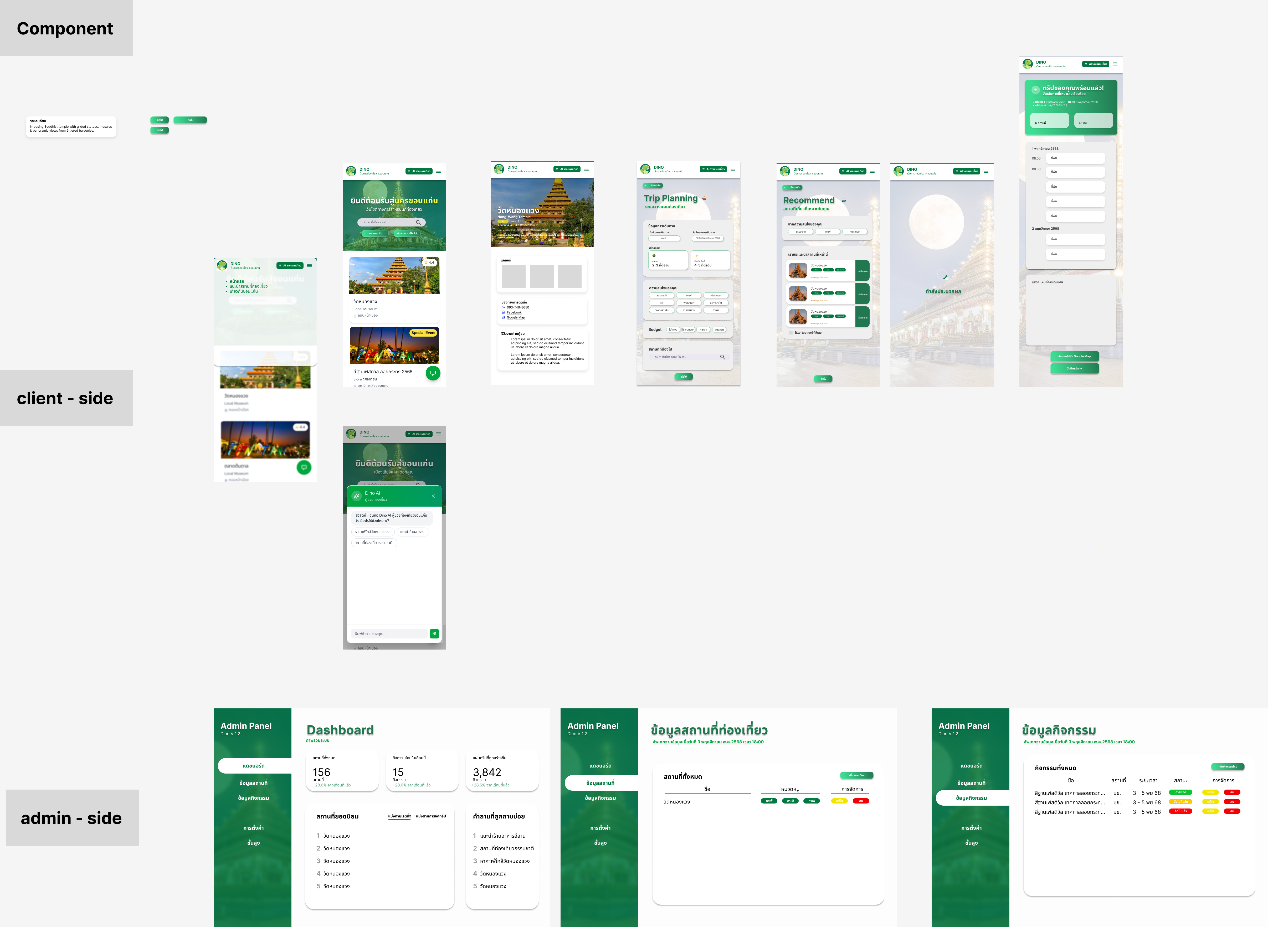
\includegraphics[width=0.95\textwidth,keepaspectratio]{images/diagram-mockup.png}
\caption{Wireframe แสดงการใช้งานระบบ}
\label{fig:mockup}
\end{figure}

\subsubsection{ส่วนของผู้ใช้งานทั่วไป (Client-Side)}

ได้รับการออกแบบในรูปแบบเว็บแอปพลิเคชัน (Web Application) แบบ Responsive ที่รองรับการใช้งานผ่านเบราว์เซอร์บนสมาร์ทโฟนเป็นหลัก เพื่อเน้นความสะดวกในการเข้าถึงข้อมูลระหว่างการเดินทาง โดยไม่ต้องติดตั้งแอปพลิเคชันแยกต่างหาก ประกอบด้วยหน้าจอและฟังก์ชันการทำงานที่สำคัญ ได้แก่

\begin{itemize}
\item หน้าหลัก (Home) และหน้ารายละเอียดสถานที่/กิจกรรม: แสดงผลข้อมูล รูปภาพ และรายละเอียดของสถานที่ท่องเที่ยว/กิจกรรมต่าง ๆ พร้อมระบบนำทาง (Navigation)
\item ระบบวางแผนการเดินทางและแนะนำสถานที่ (Trip Planning \& Recommend): ช่วยให้นักท่องเที่ยวออกแบบเส้นทาง หรือรับการแนะนำสถานที่ท่องเที่ยวที่เหมาะสมตามความต้องการ พร้อมปรับแผนได้ทันทีบนหน้าจอ (UC-06, UC-07)
\item ระบบถาม-ตอบอัตโนมัติ (แชตบอต): ทำหน้าที่เป็นผู้ช่วยเสมือนจริง ครอบคลุมข้อมูลทั่วไปเกี่ยวกับจังหวัดขอนแก่น การช่วยเหลือนักท่องเที่ยว และข้อมูลเชิงลึกเกี่ยวกับสถานที่ท่องเที่ยวที่จัดเก็บไว้ในฐานข้อมูล
\item หน้าพอยท์สะสม (Points): สแกน QR เพื่อสะสมพอยท์ และแลกของรางวัล (UC-03, UC-08)
\end{itemize}

\subsubsection{ส่วนของผู้ดูแลระบบ (Admin-Side)}

ได้รับการออกแบบในรูปแบบเว็บแอปพลิเคชัน (Web Application) เดียวกันกับฝั่งผู้ใช้งานทั่วไป (คนละเส้นทาง/Route ในโปรเจกต์เดียวกัน ไม่ใช่แอปพลิเคชันแยก) สำหรับการใช้งานบนคอมพิวเตอร์ เพื่อประสิทธิภาพในการบริหารจัดการฐานข้อมูลขนาดใหญ่ ประกอบด้วยส่วนการทำงานหลัก ได้แก่

\begin{itemize}
\item หน้ากระดานสรุปข้อมูล (Dashboard): แสดงผลภาพรวมของระบบ
\item ระบบจัดการฐานข้อมูล (Data Management): แบ่งเป็นส่วนการจัดการ ``ข้อมูลสถานที่ท่องเที่ยว'' ``ข้อมูลกิจกรรม'' ``ฐานความรู้ (Knowledge Base)'' และ ``QR/ของรางวัล'' ช่วยให้ผู้ดูแลระบบสามารถเพิ่ม ลบ ตรวจสอบสถานะ และแก้ไขปรับปรุงข้อมูลในระบบให้เป็นปัจจุบันอยู่เสมอ โดยฟอร์มจัดการกิจกรรมมีเครื่องมือช่วยดึงข้อมูลจากข้อความโพสต์ด้วย AI ประกอบอยู่ด้วย (UC-13)
\end{itemize}

% -----------------------------------------------------------
\section{การพัฒนาโปรแกรม}
% -----------------------------------------------------------

\subsection{ภาษาและเครื่องมือที่ใช้ในการพัฒนา}

\begin{enumerate}
\item \textbf{Frontend:} React 18 ร่วมกับ Vite (Build Tool) และ react-router-dom (จัดเส้นทางหน้าเว็บ) -- เว็บแอปพลิเคชันเดียว ไม่มี Native Mobile
\item \textbf{Backend (Core API):} Node.js กับ Express, เชื่อมต่อฐานข้อมูลผ่าน @supabase/supabase-js
\item \textbf{AI Service:} Python กับ FastAPI, เป็นบริการอิสระแยกจาก Core API (ไม่ได้ทำหน้าที่เป็น API Gateway ให้กัน)
\item \textbf{Database:} PostgreSQL ผ่านบริการ Supabase (Managed Service) พร้อมส่วนขยาย pgvector สำหรับ Vector Search -- ไม่มีฐานข้อมูลเวกเตอร์แยกต่างหาก (ไม่ใช่ MongoDB/Chroma)
\item \textbf{AI \& Libraries:} โมเดลภาษาขนาดใหญ่ Google Gemini (gemini-2.5-flash สำหรับ แชตบอต/Event Extraction, gemini-2.5-pro สำหรับ Trip Planner Generator/Judge) เรียกผ่าน KKU AI Gateway ที่มีรูปแบบ API แบบเดียวกับ OpenAI (ไลบรารี openai Python SDK), sentence-transformers (paraphrase-multilingual-MiniLM-L12-v2) สำหรับสร้าง Embedding ในเครื่อง
\item \textbf{API ภายนอก:} Google Places API สำหรับดึงข้อมูลตั้งต้น (Data Seeding), Serper API สำหรับค้นหาข้อมูลเสริมประกอบการสร้างคำอธิบายสถานที่ด้วย AI (UC-12)
\end{enumerate}

\subsection{โครงสร้างของโปรแกรม}

โปรเจกต์แบ่งออกเป็น 3 โฟลเดอร์หลักตามแต่ละบริการ ดังนี้

\begin{enumerate}
\item \textbf{frontend/src} -- pages/ (หน้าจอหลักของผู้ใช้งานทั่วไป เช่น HomePage, TripFormPage, TripResultPage, PointsPage, PlaceDetailPage), admin/ (แท็บจัดการข้อมูลฝั่ง Admin Portal เช่น PlacesTab, EventsTab, KnowledgeTab, QrTab), components/ (ส่วนประกอบใช้ซ้ำ เช่น ChatWidget, ImageGallery, Header), context/ (AppContext.jsx -- จัดการ State กลางของทั้งแอป), lib/ (apiClient.js, chatbotService.js -- ฟังก์ชันเรียก API)
\item \textbf{backend/src} -- routes/ (places, events, knowledgeBase, qrs, rewards -- ประกาศเป็น CRUD Router ต่อ 1 ตาราง), lib/ (crudRouter.js -- Router กลางที่สร้าง CRUD endpoint ให้ทุกตาราง, mappers.js -- แปลงข้อมูลระหว่างรูปแบบ Frontend/Database, supabaseClient.js), middleware/ (asyncHandler.js, errorHandler.js), และ scripts//supabase/migrations/ สำหรับนำเข้าข้อมูลตั้งต้นและโครงสร้างฐานข้อมูล
\item \textbf{chatbot-service/src} -- api/ (routes\_chatbot.py, routes\_tripplanner.py, routes\_events.py -- FastAPI Endpoint ของแต่ละฟีเจอร์), core/ (config.py -- ตั้งค่า Environment/โมเดล, db.py -- Supabase Client), services/rag/ (retriever.py, synonyms.py -- ค้นคืนข้อมูลด้วย Hybrid Search), services/chatbot/ (agent.py -- ประกอบ Prompt และเรียก LLM แบบ Streaming), services/trip\_planner/ (orchestrator.py, llm\_extractor.py, judge.py, models.py -- ตรรกะการสร้างและตรวจสอบแผนการเดินทาง)
\end{enumerate}

\subsection{ข้อกำหนดเฉพาะของแต่ละส่วน}

\begin{itemize}
\item \textbf{Core Backend (Node.js/Express):} ให้บริการ REST API มาตรฐานที่ /api/places, /api/events, /api/knowledge-base, /api/qrs, /api/rewards รองรับ Method GET (List), POST (Create), PUT (Update ตาม id), DELETE (ตาม id) เหมือนกันทุก Endpoint ผ่าน Router กลาง (crudRouter.js) เพื่อลดโค้ดซ้ำซ้อน
\item \textbf{AI Service (Python/FastAPI):} ให้บริการ 3 กลุ่ม Endpoint หลัก ได้แก่ POST /chat (สนทนากับ แชตบอต แบบ Streaming ผ่าน Server-Sent Events), POST /trip/llm (สร้างแผนการเดินทางด้วย AI พร้อมตรวจสอบคุณภาพด้วย LLM-as-a-Judge ก่อนตอบกลับ) และ POST /events/extract (แยกข้อมูลกิจกรรมจากข้อความโพสต์ด้วย AI)
\item \textbf{ความสัมพันธ์ระหว่างบริการ:} Frontend เรียก Core Backend และ AI Service แยกกันโดยตรง (คนละ Base URL) ทั้งสองบริการไม่เรียกหากันเอง แต่ใช้ฐานข้อมูล PostgreSQL/Supabase ร่วมกันเป็นจุดเชื่อมข้อมูล
\end{itemize}

\subsection{การติดต่อกับฐานข้อมูลและ Services}

ทั้ง Core Backend และ AI Service เชื่อมต่อฐานข้อมูล PostgreSQL ผ่าน Supabase แต่ใช้ไลบรารีคนละภาษา:

\begin{itemize}
\item \textbf{Core Backend (Node.js):} ใช้ไลบรารี @supabase/supabase-js สร้าง Client ตัวเดียว (lib/supabaseClient.js) แล้วให้ crudRouter.js เรียกใช้ผ่าน Query Builder มาตรฐาน (.select(), .insert(), .update(), .delete()) สำหรับทุกตาราง
\item \textbf{AI Service (Python):} ใช้ไลบรารี supabase (Python SDK) สร้าง Client ด้วย Service Role Key (core/db.py) สำหรับ Query ทั่วไป แต่การค้นหาความคล้ายด้วยเวกเตอร์ (ORDER BY embedding <=> query\_embedding) ไม่สามารถเขียนผ่าน Query Builder ของ supabase-py ได้โดยตรง จึงเรียกผ่านฟังก์ชัน SQL ที่ประกาศไว้ในฐานข้อมูล (match\_places, match\_knowledge\_base) ด้วยคำสั่ง supabase.rpc(...) แทน
\item \textbf{Embedding Pipeline:} การแปลงข้อความเป็นเวกเตอร์ทำผ่านสคริปต์แยกต่างหาก (scripts/embed\_content.py) ที่ต้องรันด้วยตนเองหลังข้อมูลสถานที่/ฐานความรู้เปลี่ยนแปลง เนื่องจากยังไม่ได้เชื่อมเป็น Trigger อัตโนมัติกับการบันทึกข้อมูลผ่าน Admin Portal
\end{itemize}

% -----------------------------------------------------------
\section{การทดสอบระบบ}
% -----------------------------------------------------------

\subsection{วิธีการทดสอบ}

\subsubsection{การทดสอบยอมรับจากผู้ใช้ (User Acceptance Testing: UAT)}

ทดสอบกับกลุ่มผู้ใช้เป้าหมาย (นักศึกษา/นักท่องเที่ยวในจังหวัดขอนแก่น) โดยใช้เกณฑ์ประเมินด้านความง่ายในการใช้งาน (Ease of Use) ความพึงพอใจ (Satisfaction) และความเข้าใจในการนำเสนอข้อมูล

\subsubsection{วิธีการประเมินผลของการวิจัย (LLM as a Judge)}

เพื่อให้มั่นใจว่าแผนการเดินทางที่ระบบสร้างขึ้นด้วย AI มีความถูกต้องและใช้งานได้จริง งานวิจัยนี้ได้พัฒนากลไกการตรวจสอบผลลัพธ์โดยใช้ LLM อีกตัวหนึ่ง (gemini-2.5-pro) ทำหน้าที่เป็น ``ผู้ประเมิน'' (Judge) แทนการเขียนฟังก์ชันตรวจสอบแบบตายตัว โดยเป็นขั้นตอนที่ทำงานอัตโนมัติอยู่เบื้องหลังทุกครั้งที่มีการสร้างแผนการเดินทาง (UC-06) ไม่ใช่กระบวนการที่ผู้ใช้เห็นหรือสั่งงานเอง เกณฑ์การประเมินและกลไกการทำงานจริงมีดังนี้

\begin{table}[H]
\centering
\caption{เกณฑ์การประเมินคุณภาพแผนการเดินทางด้วยเทคนิค LLM-as-a-Judge (ตามที่พัฒนาจริงใน judge.py)}
\label{tab:llm_judge}
\begin{tabular}{|p{5.2cm}|p{2.8cm}|p{6cm}|}
\hline
\textbf{เกณฑ์} & \textbf{รูปแบบผลลัพธ์} & \textbf{ปัจจัยที่ใช้พิจารณา} \\
\hline
1. Pacing (pacing\_ok) & Boolean (ผ่าน/ไม่ผ่าน) -- เกณฑ์บังคับ & ไม่มีมื้ออาหารหลัก 2 มื้อติดกันโดยไม่มีกิจกรรมอื่นคั่น และความหนาแน่นของกิจกรรมเหมาะสมกับ Pace ที่ผู้ใช้เลือก \\ \hline
2. Intent Match (intent\_match\_ok) & Boolean (ผ่าน/ไม่ผ่าน) -- เกณฑ์บังคับ & แผนสะท้อนความสนใจ สถานที่ต้องไป (Must-go) และระดับงบประมาณที่ผู้ใช้ระบุจริงหรือไม่ \\ \hline
3. Score & ตัวเลข 0.0--1.0 & คะแนนคุณภาพโดยรวมจาก LLM \\
\hline
\end{tabular}
\end{table}

การตัดสิน ``ผ่าน'' (passed) คำนวณฝั่ง Backend เอง (ไม่เชื่อค่าจาก LLM โดยตรง) โดยต้องผ่านเงื่อนไขทั้ง 3 ข้อพร้อมกัน คือ pacing\_ok เป็นจริง และ intent\_match\_ok เป็นจริง และ Score $\geq$ 0.45 (PASS\_SCORE\_THRESHOLD) ค่า 0.45 นี้ปรับลดมาจาก 0.6 เนื่องจากผลทดสอบจริงในช่วงแรกพบว่าโมเดล Judge ที่ใช้ขณะนั้น (gemini-2.5-flash) แทบไม่เคยให้คะแนนเกิน 0.5 แม้แผนจะผ่านเกณฑ์บังคับทั้งสองข้อแล้วก็ตาม ค่านี้จึงจำเพาะกับพฤติกรรมของโมเดลรุ่นที่ทดสอบ และจำเป็นต้องทดสอบซ้ำหากเปลี่ยนโมเดล Judge ในอนาคต

หากแผนไม่ผ่านเกณฑ์ ระบบจะนำข้อคิดเห็น (feedback) ที่ Judge ให้กลับไปแนบใน Prompt แล้วสั่งให้ LLM สร้างแผนใหม่อีกครั้ง วนซ้ำได้สูงสุด MAX\_JUDGE\_ATTEMPTS รอบ หากครบจำนวนรอบแล้วยังไม่ผ่าน ระบบจะส่งแผนล่าสุดที่ได้กลับไปให้ผู้ใช้ โดยไม่บล็อกการใช้งาน และหากการเรียก Judge เกิดข้อผิดพลาดทางเทคนิค (เช่น เรียก API ไม่สำเร็จ) ระบบจะถือว่า ``ผ่าน'' โดยอัตโนมัติ (Fail-Open) เพื่อไม่ให้ความผิดพลาดของขั้นตอนตรวจสอบไปปิดกั้นผู้ใช้จากผลลัพธ์ที่สร้างเสร็จแล้ว

นอกจากตัดสินผ่าน/ไม่ผ่านแล้ว Judge ยังสร้างข้อความ rationale เป็นคำอธิบายภาษาไทยสั้น ๆ อธิบายเหตุผลของแผนในเชิงบวกให้ผู้ใช้เห็นประกอบผลลัพธ์ (เช่น เหตุผลที่จัดร้านอาหารให้เว้นระยะ) โดยไม่เปิดเผยคะแนนหรือกระบวนการตรวจสอบภายในให้ผู้ใช้ทราบ

\subsection{ผลการทดสอบ}

ผลการทดสอบและความคืบหน้าล่าสุดของแต่ละส่วนของระบบ ณ ช่วงเวลาจัดทำรายงานฉบับนี้ แสดงไว้ในบทที่ 5 หัวข้อ ``สรุปผลการดำเนินโครงงาน''